\chapter{Introducción a Numpy\\ Introduction to Numpy}\index{Numpy} \index[eng]{Numpy}
\chaptermark{Intro. a Numpy \textreferencemark\ Intro to Numpy}
\epigraph{When the going gets tough, the tough get going}{Popular Witticism (US)}
\begin{paracol}{2}
\section{Numpy: un paquete de Python para cálculo nu\-mérico}
En el capítulo \ref{ch:intpr}, vimos cómo importar mó\-dulos de python en un script o directamente en el terminal de Ipython, de modo que podamos reutilizar el código contenido en ellos. Numpy es un libraría de python que contiene funciones y variables específicamente diseñadas para el cálculo numérico. Está estructurada en forma de módulos y submódulos de modo que para utilizarla en nuestros programas basta  importarla en nuestros script, importar sus submodulos o importar sus funciones.
La base de Numpy la constituyen objetos y operaciones algebráicas. En esta sección vamos a repasar algunos conceptos fundamentales de  álgebra lineal y cómo pueden manejarse empleando Python. No daremos definiciones precisas ni tampoco demostraciones, ya que tanto unas como otras se verán en detalle en la asignatura de álgebra.

\paragraph{Matrices.} Desde un punto de vista funcional definiremos una matriz como una tabla bidimensional de números ordenados en filas y columnas,
\switchcolumn

\section{Numpy: a Python library for scientific computing}
In chapter \ref{ch:intpr}, we have seen how to import Python modules to a script or to the Ipython console. In this way, we can reuse the code available in the modules. Numpy is a Python library with functions and variables specifically intended to perform scientific computing. Numpy is structured in modules and submodules so that we can import the whole library, its submodules, or just any of its functions into our scripts. The background of Numpy is built of algebraic objects and operations. In this section, we will review some fundamental notions of linear algebra and how to deal with them using Numpy. We will not provide formal definitions or demonstrations because both will be studied in detail in algebra during the next term.
\paragraph{Matrices} From a functional perspective, we will define a matrix as a table of numbers ordered by rows and columns,
\end{paracol}

\begin{equation*}
A=
\begin{pmatrix}
1& \sqrt{2}& 3.5& 0\\
-2& \pi& -4.6& 4\\
7& -19& 2.8& 0.6
\end{pmatrix}
\end{equation*}

\begin{paracol}{2}
Cada línea horizontal de números constituye una \emph{fila} de la matriz y cada línea vertical una \emph{columna} de la misma.

A una matriz con $m$ filas y $n$ columnas se la denomina matriz de orden $m\times n$. $m$ y $n$ son la dimensiones de la matriz y se dan siempre en el mismo orden: primero el número de filas y después el de columnas. Así, la matriz $A$ del ejemplo anterior es una matriz $3\times 4$, y como esta formada por números reales se dice que $A\in\mathbb{R}^{3\times 4}$. El orden de una matriz expresa el tamaño de la matriz.

Dos matrices son iguales si tienen el mismo orden, y los elementos que ocupan en ambas matrices los mismo lugares son iguales.

Una matriz es cuadrada, si tiene el mismo número de filas que de columnas. Es decir es de orden $n\times n$.

Mientras no se diga expresamente lo contrario, emplearemos letras mayúsculas $A, B, \cdots$ para representar matrices. La expresión $A_{m\times n}$ indica que la matriz $A$ tiene dimensiones $m \times n$. Para denotar los elementos de una matriz, emplearemos la misma letra en minúsculas empleada para nombrar la matriz, indicando mediante subíndices, y siempre por este orden, la fila y la columna a la que pertenece el elemento. Así por ejemplo $a_{ij}$ representa al elemento de la matriz $A$, que ocupa la fila $i$ y la columna $j$.
\switchcolumn
Each horizontal line of numbers forms a matrix row, and each vertical line a matrix column.
A matrix with $m$ rows and $n$ columns is denoted as a matrix of order $m\times n$. $m$ and $n$ are the matrix dimensions, and they are always defined in the same order: first, the number of rows and then the number of columns. So matrix $A$ in the example above is a $3\times 4$ matrix, and as it is built of real numbers, we say that $A\in \mathbb{R}^{3\times 4}$. The matrix order defines the size of the matrix.

Two matrices are equal if they have the same order and the elements located in both matrices in the same place are equal. A matrix is square when it has the same number of rows and columns. That is, it is an $n\times n$ matrix.

From now on, we will use capital letters $A,\ B,\cdots$ to name matrices. The expression $A_{m\times n}$ means that matrix $A$ has dimensions $m\times n$. We will refer to the elements of a matrix using the same letter used to name the matrix but in lowercase and using subindexes to indicate the row and column the element belongs to. The first subindex always represents the row, and the second is the column. For instance, $a_{ij}$ Represents the matrix $A$ element that belongs to row $i$ and to column $j$.
\end{paracol}
\begin{equation*}
A=
\begin{pmatrix}
1& \sqrt{2}& 3.5& 0\\
-2& \pi& -4.6& 4\\
7& -19& 2.8& 0.6
\end{pmatrix}
\rightarrow a_{23}=-4.6
\end{equation*}
\begin{paracol}{2}
\paragraph{vectores}
A una matriz compuesta por una sola fila, la denominaremos vector fila. A una matriz compuesta por una sola columna la denominaremos vector columna. Siempre que hablemos de un vector, sin especificar más, entenderemos que se trata de un vector columna.\footnote{Esta identificación de los vectores como vectores columna no es general. La introducimos porque simplifica las explicaciones posteriores.} Para representar vectores, emplearemos letras minúsculas. Para representar sus elementos añadiremos a la letra que representa al vector un subíndice indicando la fila a la que pertenece el elemento.
\switchcolumn
We call a matrix formed by a single row a row vector. We call a matrix formed by a single column a column vector. Whenever we speak of a vector without further specification, we consider it a column vector.\footnote{This identification of a vector with a column vector is by no means general. We introduce it because it simplifies the exposition.}. To name vectors, we will use lowercase letters. To name the elements of a vector, we will add a subindex to the letter representing the vector to show the row the element belongs to. 
\end{paracol}
\begin{equation*}
a=
\begin{pmatrix}
a_1\\
a_2\\
\vdots \\
a_i\\
\vdots \\
a_n
\end{pmatrix}
\end{equation*}
\begin{paracol}{2}
Podemos asociar los puntos del plano con los vectores de dimensión dos. Para ello, usamos una representación cartesiana, en la que los elementos del vector son los valores de las coordenadas $(x,y)$ del punto del plano que representan. Cada vector se representa gráficamente mediante una flecha que parte del origen de coordenadas y termina en el punto $(x,y)$ representado por el vector. La figura \ref{fig:vectores} representa los vectores,
\switchcolumn
We can establish a relationship between the plane points and two-dimensional vectors. To do so, we use a Cartesian representation, in which the elements of a vector are the $(x,y)$ coordinates of the point of the plane they represent. Each vector is drawn using an arrow that starts at the origin of the coordinates and ends at the point $(x,y)$ represented by the vector. Figure \ref{fig:vectores} represents vectors, 
\end{paracol}
\begin{equation*}
a=
\begin{pmatrix}
1\\
2
\end{pmatrix},
b=
\begin{pmatrix}
2\\
-3
\end{pmatrix},
c=
\begin{pmatrix}
0\\
-2
\end{pmatrix}
\end{equation*}


\begin{figure}[h]
\centering
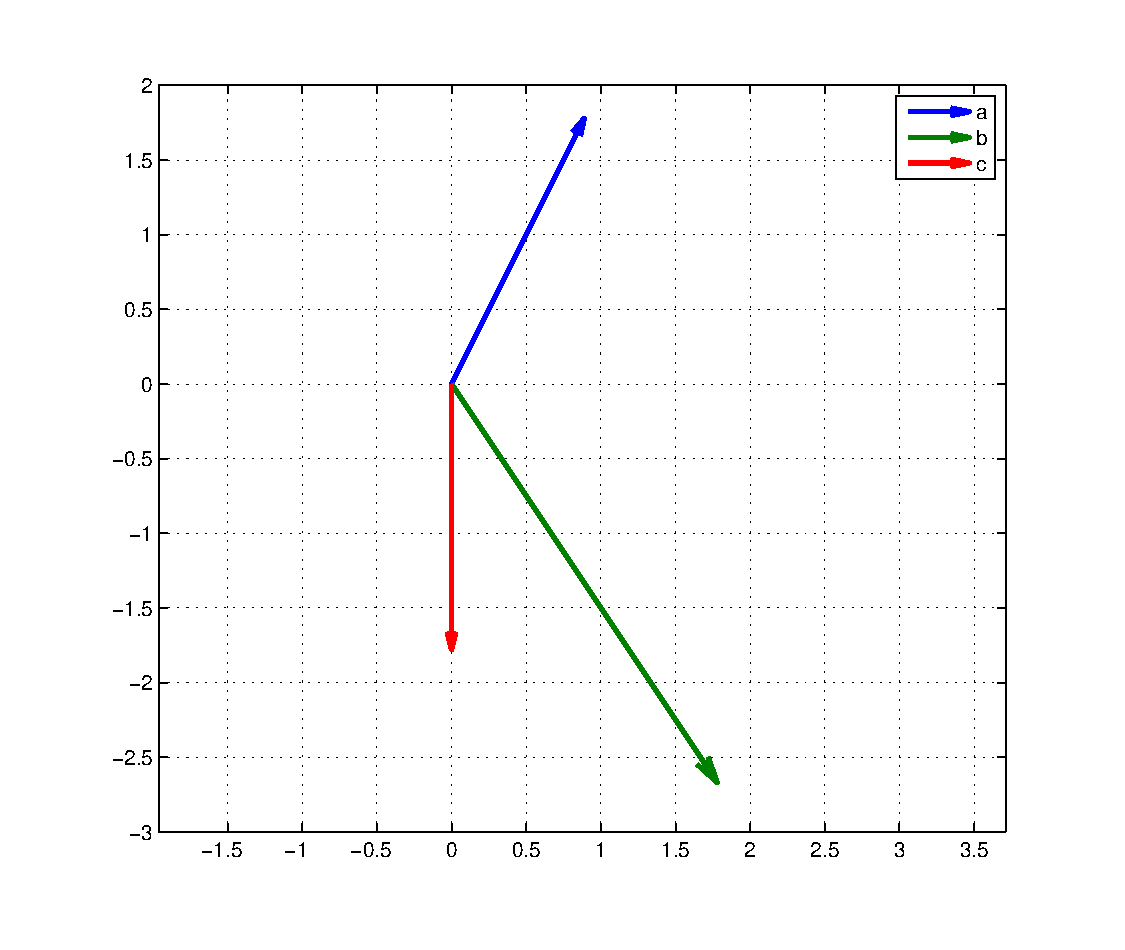
\includegraphics[width=7cm]{vectores.eps}
\bicaption{Representación gráfica de vectores en el plano}{Graphic of vectors on the plane}
\label{fig:vectores}
\end{figure}

\begin{paracol}{2}
De modo análogo, podemos asociar vectores de dimensión tres con puntos en el espacio tridimensional. En este caso, los valores de los elementos del vector corresponden con la coordenadas $(x,y,z)$ de los puntos en el espacio. La figura \ref{fig:vectores3} muestra la representación gráfica en espacio tridimensional de los vectores,
\switchcolumn
Likewise, we can associate vectors of dimension three with points in the 3D space. In this case, the vector elements represent the coordinates $(x,y,z)$ of the points in the space. Figure \ref{fig:vectores3} shows a graphic representation of vectors,
\end{paracol}
\begin{equation*}
a=
\begin{pmatrix}
1\\
2\\
1
\end{pmatrix},
b=
\begin{pmatrix}
2\\
-3\\
-1
\end{pmatrix},
c=
\begin{pmatrix}
0\\
-2\\
1
\end{pmatrix}
\end{equation*}

\begin{figure}[h]
\centering
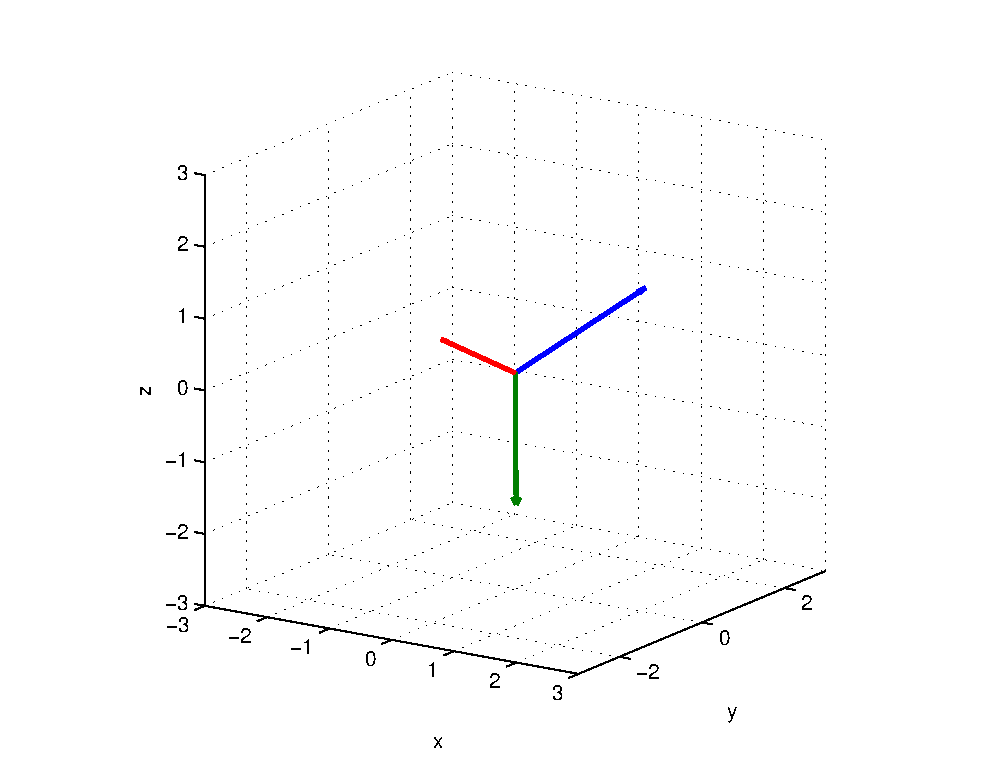
\includegraphics[width=9cm]{vectores3.eps}
\bicaption{Representación gráfica de vectores en el espacio 3D}{Graphic of vector in the 3D space}
\label{fig:vectores3}
\end{figure}
\begin{paracol}{2}
Evidentemente para vectores de mayor dimensión, no es posible obtener una representación gráfica. Si embargo muchas de las propiedades geométricas, observables en los vectores bi y tridimensionales, pueden extrapolarse a vectores de cualquier dimensión.

\subsection{Vectores y matrices en\\ Numpy.} \index{Vectores!en Numpy} \index{Matrices!en Numpy} 
\paragraph{Matrices.} Una de las característica más interesantes de Numpy, es la posibilidad de crear fácilmente matrices. Se pueden crear de diferentes maneras, la más elemental de todas ellas, emplea la funcion de Numpy \mintinline{python}{array} aplicada a una lista de filas de la matriz que se quiere construir. Cada fila debe ser a su vez una lista de números. Evidentemente, para que se pueda construir la matriz, todas las filas deben tener el mismo número de elementos. El siguiente ejemplo muestra como construir una matriz de dos filas y tres columnas,

\switchcolumn 
Obviously, it is impossible to get a graphic representation for vectors of larger dimensions. Nevertheless, many geometrical properties owned by 2D and 3D vectors can be applied to vectors of whatever dimension.

\subsection{Vetors and matrices in Numpy.}\index[eng]{Vectors! in Numpy}\index[eng]{Matrices! in Numpy}
\paragraph{Matrices.} One interesting feature of numpy is that it allows us to create matrices easily. There are several methods to create them, but using the Numpy function \mintinline{python}{array} with a Python list with the rows of the matrix we want to build is probably the easiest method. Each row should be, in turn, a list of numbers, i.e., matrix elements. Of course, to build a matrix all rows should have the same number of elements. The following example shows how to build a matrix of two rows and three columns.
\end{paracol}

\begin{center}
    \begin{minipage}{0.4\textwidth}
    \begin{minted}{python}
In [3]: import numpy as np

In [4]: A = np.array([[1,2,3],[4,5,6]])

In [5]: print(A)
[[1 2 3]
 [4 5 6]]

In [6]: L = [[1,2,3],[4,5,6]]

In [7]: B = np.array(L)

In [9]: print(L)
[[1, 2, 3], [4, 5, 6]]

In [10]: print(B)
[[1 2 3]
 [4 5 6]]
 \end{minted}
\end{minipage}
 \end{center}
\begin{paracol}{2} 
Lo primero que hacemos es importar Numpy, lo importamos usando como alias la abreviatura np, porque es más cómodo a la hora de llamar a funciones específicas de Numpy.  Hemmos construido dos matrices iguales \mintinline{python}{A} y \mintinline{python}{B}. En el primer caso hemos creado directamente dentro de la llamada a la función \mintinline{python}{array}, la lista a partir de la cual construimos la matriz. En el segundo caso, hemos construido primero una lista \mintinline{python}{L}, y luego hemos empleado dicha lista como variable de entrada de la función \mintinline{python}{array}. Si nos fijamos en las líneas [9] y [10], vemos como Python distingue la lista ---todos sus elementos aparacen representados en la misma línea---, de la matriz en la que cada fila ocupa una línea distinta. Podemos construir matrices a partir de listas y variables ya definidas, siempre que seamos coherentes con el criterio de que cada fila se cree a partir de una lista y que todas las filas tengan los mismos elementos,
\switchcolumn
First, we import Numpy; we do it using \mintinline{python}{np} as an alias. The reason is that \mintinline{python}{np} is shorter than \mintinline{python}{numpy}, and it eases the calls to specific Numpy functions. We have built two identical matrices \mintinline{python}{a} and \mintinline{python}{B}. In the first case, we have straightforwardly created the list needed to make the matrix inside the call to the function \mintinline{python}{array}. In the second case, we first created a list \mintinline{python}{L}, and then we used it as an input variable to the function \mintinline{python}{array}. Focusing on lines [9] and [10], we see how Python can tell a list and a matrix apart. For a list, Python represents all elements in the same line. For a matrix, each row is written in a different line.
We can build matrices from lists and variables already defined as long as we follow the criteria that each row be created from a list and all rows have the same number of elements,  
\end{paracol}
\begin{center}
    \begin{minipage}{0.4\textwidth}
        \begin{minted}{python}
In [23]: a =1; b= 2; c =3

In [24]: d =[4,5,6]

In [25]: C = np.array([[a,b,c],d])

In [26]: print(C)
[[1 2 3]
 [4 5 6]]

In [27]: C = np.array([[a,b,c],d,[7,8,9]])

In [28]: print(C)
[[1 2 3]
 [4 5 6]
 [7 8 9]]
        \end{minted}
    \end{minipage}
\end{center}
\begin{paracol}{2}
\paragraph*{Indexación.} \index{Numpy!indexación}Al igual que se hace en álgebra, Numpy es capaz de referirse a un elemento cualquiera de una matriz empleando índices para determinar su posición (fila y columna) dentro de la matriz.
\switchcolumn
\paragraph{Indexing}\index[eng]{Numpy!Indexing} As in algebra, in NUmpy is also possible to refer any element of a matrix using indexes to indicate its position (row and column) in the matrix. 
\end{paracol}
\begin{equation*}
A=
\begin{pmatrix}
a_{11}&a_{12}&a_{13}\\
a_{21}&a_{22}&a_{23}\\
a_{31}&a_{32}&a_{33}
\end{pmatrix}
\end{equation*}

\begin{paracol}{2}
Sin embargo,  el criterio para referirse a un elemento concreto de una matriz, en Numpy está heredado de las listas: se indica el nombre de la variable que contiene la matriz y a continuación, entre corchetes y separados por una coma, el índice de su fila y después él de su columna \textbf{pero empezando a contar desde $0$}. Es decir, la primera fila de una matriz de dimensión $m\times n$ es la fila $0$ y la última es la fila $m-1$. De modo análogo su primera columna es la $0$ y su última columna es la $n-1$,
\switchcolumn
However, the Numpy criteria to refer to a specific element inside a matrix has been borrowed from Python Lists: we write the name of the matrix followed by the row and column indexes of the element we are interested in, enclosed in a square bracket and separated by a comma. The point is that we \textbf{count the rows and columns starting at $0$}. Thus, the first row of a matrix with dimensions $m\times n$ is the row $0$, and the last is the row $m-1$. Likewise, its first column is column $0$, and the last one is column $n-1$, 
\end{paracol}
\begin{center}
    \begin{minipage}{0.3\textwidth}
        \begin{minted}{python}
In [31]: print(C)
[[1 2 3]
 [4 5 6]
 [7 8 9]]

In [32]: C[1,2]
Out[32]: 6

In [33]: C[0,0]
Out[33]: 1
        \end{minted}
    \end{minipage}
\end{center}

\begin{paracol}{2}
Numpy puede seleccionar dentro de una matriz no solo elementos aislados, sino también submatrices completas. 
Para ello, emplea un símbolo reservado, el símbolo \emph{dos puntos} $:$. Este símbolo se emplea para recorrer valores desde un valor inicial hasta un valor final, con un incremento o paso fijo. La sintaxis es: \mintinline{python}{inicio:fin:paso}. Es importante tener en cuenta que Numpy detendrá la cuenta en el valor \mintinline{python}{stop-step}. Además, si no indicamos el tamaño del paso, Numpy tomará por defecto un paso igual a uno. En este caso basta emplear \mintinline{python}{start:stop}
\switchcolumn
Inside a matrix, Numpy can select single elements and whole submatrices. To do so, it uses the colon : symbol as a special symbol. Using a fixed step, we use this symbol to cover a set of values from a start (initial) value to a stop (final) one. The syntax is simple: \mintinline{python}{start:stop:step}. Beware! Numpy will stop the count in the step \mintinline{python}{stop-step}. Besides, if we leave apart the step size, Numpy will take a step equal to one. In this case, the expression is just \mintinline{python}{start:stop}
\end{paracol}

\begin{center}
        \begin{minted}{python}
In [87]: D = numpy.array([[1.,2.,3.],[4.,5.,6.],[-2,-3,0],[3,2,1]])

In [88]: print(D)
[[ 1.  2.  3.]
 [ 4.  5.  6.]
 [-2. -3.  0.]
 [ 3.  2.  1.]]

In [90]: D[0:1,0:3]
Out[90]: array([[1., 2., 3.]])

In [91]: D[0:2,0:2]
Out[91]: 
array([[1., 2.],
       [4., 5.]])

In [92]: D[2:3,1:2]
Out[92]: array([[-3.]])

In [93]: D[3:4,0:3]
Out[93]: array([[3., 2., 1.]])

In [94]: D[0:4,0:3]
Out[94]: 
array([[ 1.,  2.,  3.],
       [ 4.,  5.,  6.],
       [-2., -3.,  0.],
       [ 3.,  2.,  1.]])

In [95]: D[0:4,2:3]
Out[95]: 
array([[3.],
       [6.],
       [0.],
       [1.]])
       \end{minted}
\end{center}

\begin{paracol}{2}
La línea [90], extrae un vector fila con los elementos de la primera fila de la matriz \mintinline{python}{D}. La fila [91] extrae una matriz de dimension $2\times 2$ con los cuatro elementos de la esquina superior izquierda de la matriz original. La fila [92] extrae un único elemento pero sigue siendo una matriz de dimensión $1 \times 1$, por tanto es distinto que si empleamos la indexación directa del elemento: \mintinline{python}{D[2,1]}. La línea [93] nos devuelve un vector fila con la última fila de la matriz. La línea [94], nos devuelve de nuevo la matriz entera. Por último la línea [95] nos devuelve un vector columna con la primera columna de la matriz.

Hemos dicho que la línea [95] nos devuelve un vector columna. Bueno, sí y no; vamos a verlo más despacio.

\paragraph{Vectores.}
Cuando introducimos los vectores, distinguimos entre vectores filas y columna, definiéndolos como matrices de una sola fila o una sola columna. Sin embargo, en Numpy, se sigue un criterio distinto que permite generalizar el concepto de matriz asociándolo con el de tensor. Sin entrar en detalles\footnote{Una definición formal del concepto de tensor, queda fuera del alcance de estos apuntes.}, podemos decir que un tensor es un objeto algebráico caracterizado por dos parámetros; el orden y la dimensión. Así un escalar $a \in \mathbb{R}$ es un tensor de orden cero. Un vector $b \in \mathbb{R}^n$ es un tensor de orden 1 y dimesión $n$. Una matriz $A \in \mathbb{R}^{m\times n}$ Es un tensor de orden dos y dimensiones $m,n$. Un tensor de orden 3, $T \in \mathbb{R}^{n\times m \times l}$, etc. Podemos asociar el orden al número mínimo de índices que necesitamos para definir de forma unívoca los elementos de un Tensor: para un escalar, no nos hace faltar ningún indice, solo tenemos un elemento que es el propio escalar, por tanto le asociamos orden cero. Para un vector es suficiente emplear un índice para definir sus elementos, $b=(b_i),\ i=1,\cdots, n$, $b \in \mathbb{R}^n$. Para una matriz necesito dos índices, $A=(a_{ij}),\ i =1, \cdots n, j = 1,\ \cdots, m$, $A \in \mathbb{R}^{n\times m}$. Para un tensor de orden tres necesitaría tres índices, $T=(T_{ijk}),\ i =1,\cdots, n,\ j =1,\cdots m,\ k = 1,\cdots, l$, $T\in \mathbb{R}^{n\times m \times l}$ y así sucesivamente. Numpy permite definir estructuras de cualquier orden y dimensión que queramos. Pero nosotros nos vamos a limitar a vectores (orden 1) y matrices (orden 2). ¿Tiene sentido entonces distiguir entre vectores fila y columna? Solo si consideramos siempre los vectores como matrices (orden 2) y dimesiones $1\times n$ (vector fila) ó $n \times 1$ (vector columna). Para Numpy, sin embargo, vectores y matrices son estructuras de distinto orden. Veamos con algunos ejemplo cómo se diferencian. Para verlo mejor podemos emplear la propiedad \mintinline{python}{shape} de los arrays en numpy, Dicha propiedad nos devuelve una tupla con las dimensiones del array, el número de elementos que contine la tupla nos da el orden,
\switchcolumn
Line [90] extracts a row vector from the first row of matrix \mintinline{python}{D}. Line [91] extracts a $2\times 2$ matrix using the four elements located on the left-up corner of the original, \mintinline{python}{D}, matrix. Line [92] extracts a single matrix element, but notice that it takes the form of a $1\times 1$ matrix. Thus, this result is different than the result achieved when we directly use the indexes of the element: \mintinline{python}{D[2,1]}. Lain [93] returns a row vector with the elements of the matrix's last row. Lastly, line [95] returns a column vector with the elements of the matrix's last column.

We have said that line [95] returns a column vector. well, yes and not; let's see it in more detail.

\paragraph{Vectors.} When we introduced vectors in the previous section, we made a distinction between row and column vectors, defining them as matrices with a single row or a single column. Nevertheless, Numpy follows another criterion that allows us to generalise the idea of matrix linking it with the concept of tensor. we do not get into details\footnote{A formal definition of tensors is far beyond the scope of these notes.} and simply say that a tensor is an algebraic object defined by two parámeters, its order, and its dimension. So, a scalar $a \in \mathbb{R}$ is a tensor of order zero. A vector $b \in \mathbb{R}^n$ is a tensor of order one and dimension $n$. A matrix $A\in \mathbb{R}^{m\times n}$ is a tensor of order two and dimensions $m,n$. A third order tensor, $T\in\mathbb{R}^{n\times m\times l}$, etc. We can relate the order with the minimum number of indexes we need to univocally define the tensor element: for a scalar, we don't need an index at all; we have only a single element, the scalar itself. For this reason, we associate scalars with a zero-order tensor. For a vector, it is enough to use a single index to define its elements, $b=(b_i), i = 1,\cdots, n,\ b \in \mathbb{R}^n$. For a matrix, we need two indexes, $A = (a_{ij}), i =1,\dots,n,\ j = 1,\dots,m,\ A \in \mathbb{R}^{n\times m}$. For third-order tensors, we need three indexes, $T=(T_{ijk}),\ i =1,\cdots, n,\ j =1,\cdots m,\ k = 1,\cdots, l$, $T\in \mathbb{R}^{n\times m \times l}$ and so on. In Numpy, we can define structures of whatever order and dimensions we want, but we will only use vectors (order 1) and matrices (order 2). Has, then, any sense to distinguish between row and column vector? Only if we always consider vectors as matrices (order 2) and dimensions $1\times n$ (row vector) or $n\times 1$ (column vector). For Numpy, however, vectors an matrices are structures of different order. Let's see some examples of their differences. To appreciate it better we can use the Numpy arrays attribute \mintinline{python}{shape}, which gives us a tuple containing the dimensions of the array. The number of elements of the tuple tells us the order of the array,     
\end{paracol}
\begin{center}
    \begin{minipage}{0.3\textwidth}
    \begin{minted}{python}
In [23]: D
Out[23]: 
array([[ 1.,  2.,  3.],
       [ 4.,  5.,  6.],
       [-2., -3.,  0.],
       [ 3.,  2.,  1.]])

In [24]: D.shape
Out[24]: (4, 3)

In [25]: D[1,1]
Out[25]: 5.0

In [26]: D[1,1].shape
Out[26]: ()

In [27]: D[1,1:2]
Out[27]: array([5.])

In [28]: D[1,1:2].shape
Out[28]: (1,)
\end{minted}
\end{minipage}
\end{center}
\begin{center}
    \begin{minipage}{0.3\textwidth}
    \begin{minted}{python}
In [29]: D[1:2,1:2]
Out[29]: array([[5.]])

In [30]: D[1:2,1:2].shape
Out[30]: (1, 1)
    \end{minted}
        
    \end{minipage}
\end{center}

 \begin{paracol}{2}
 Empezamos con la matriz \mintinline{python}{D} de ejemplos anteriores. Para obtener sus dimensiones empleamos \mintinline{python}{D.shape}. El resultado es una tupla compuesta de dos elementos, puesto que es una matriz y, por tanto su orden es dos. El primer elemento no da la dimensión de sus columnas, es decir, el número de filas. El segundo elemento nos da la dimensión de sus filas, es decir el número de columnas. 
 
 En la línea [25] extraemos el elemento que ocupa la posición $[1,1]$. En la [26] cuando tratamos de obtener sus dimensiones, nos da una tupla vacía, porque es un escalar y su orden es cero. En la línea [27] le hemos pedido a Numpy que nos de los elementos de la fila $1$ de la matriz \mintinline{python}{D} que ocupan las columnas desde la $1$ hasta la $1$. Es decir, hacemos referencia al mismo elemento de la matriz, sin embargo el resultado no es exáctamente el mismo. Nos ha devuelto un array con el elemento seleccionado. Cuando el la línea [28] pedimos sus dimensiones, obtenemos una tupla con un único elemento \mintinline{python}{(1,)}. Es decir, el orden del array es $1$, se trata de un vector, y tiene de dimensión $1$, el vector solo tiene un elemento. 
 
 Por último, en la línea [29] volvemos a pedir a Python que nos de los elementos de la matriz \mintinline{python}{D}, que ocupan las filas desde la $1$ hasta la $1$ y las columnas desde la $1$ hasta la $1$, el resultado es ahora una matriz, podemos ver en la línea \mintinline{python}{out [29]} que el numero $5$ aparece ahora encerrado entre dos pares de corchetes. Cuando en la línea [30], preguntamos por su \mintinline{python}{shape}, nos devuelve una tupla con dos elementos --el orden del array es $2$, puesto que se trata de una matriz-- y sus dimensiones son una fila y una columna, puesto que la matriz solo tiene un elemento.  

 Vamos a completar nuestro estudio de los arrays en Python, extrayendo ahora partes más grandes de la misma matriz \mintinline{python}{D},
 \switchcolumn
 We begin with the same matrix \mintinline{python}{D} we use in previous examples. To get its dimensions, we use \mintinline{python}{D.shape}. The result is a tuple of two elements because it is a matrix, and thus, its order is two. The first element gives us its column dimension, that is, its number of rows. The second element is its row dimension, that is, its number of columns.

 In line [25] we extract the element located at position $[1,1]$. In line [26] when we try to get its dimension, Numpy returns an empty tuple because it is a scalar and its order is zero. In line [27], we ask Numpy that retrieve the elements of row $1$ of the matrix \mintinline{python}{D} that fill the columns $1$ to $1$. Thus, we are making reference to the same element of the matrix as in the previous case. However, the result is not exactly the same. Numpy retrieves an array with the selected element. When we ask for its dimensions in line [28] we get a tuple with a single element \mintinline{python}{(1,)}. Then, the order of the array is one. It is a vector with a single element.

 Finally, in line [29], we ask Numpy to retrieve the elements of matrix \mintinline{python}{D} with fill the rows from $1$ to $1$ and the columns from $1$ to $1$. Thus, the result is now a matrix, We can see in line \mintinline{python}{out [29]} that the number $5$ is enclosed in two pair of square brackets. When in line [30], we ask for its \mintinline{python}{shape}, we get a tuple with two elements  --now the order of the array is two, because it is a matrix-- and their dimension are one row and one column as far as the matrix has a single element.

 We are going to complete our study on Numpy arrays, extracting larger parts of the same matrix, 
 \end{paracol}
\begin{center}
 \begin{minipage}{0.3\textwidth}
    \begin{minted}{python}
In [9]: D
Out[9]: 
array([[ 1.,  2.,  3.],
       [ 4.,  5.,  6.],
       [-2., -3.,  0.],
       [ 3.,  2.,  1.]])

In [10]: D[1,:]
Out[10]: array([4., 5., 6.])

In [11]: D[:,1]
Out[11]: array([ 2.,  5., -3.,  2.])
    
In [12]: D[1:2,:]
Out[12]: array([[4., 5., 6.]])
\end{minted}
\end{minipage}
\end{center}
\begin{center}
 \begin{minipage}{0.3\textwidth}
    \begin{minted}{python}
In [13]: D[:,1:2]
Out[13]: 
array([[ 2.],
       [ 5.],
       [-3.],
       [ 2.]])
    \end{minted}
\end{minipage}
\end{center}
\begin{paracol}{2}
En el primer caso, línea [10], hemos extraido toda la segunda fila de la matriz \mintinline{python}{D}, el resultado es un vector, por tanto tiene orden $1$ y dimensión $3$. En la línea [11] hemos extraido la primera columna y el resultado es de nuevo un vector, por tanto tiene orden $1$ y la dimensión esta vez $4$. En la línea [12] extraemos todas las columnas de las filas que van desde la segunda hasta la segunda. El resultado es una matriz, ya que el orden del array extraído es $2$, y la dimensiones será $1$ para las filas y $3$ para las columna. Es lo más parecido a un vector 'fila' que podemos obtener con Numpy. Por último, en la línea [13], extraemos todas las filas de las columnas que van desde la segunda hasta la segunda. El resultado es de nuevo una matriz, porque el array extraido tiene orden dos, pero las dimensiones son ahora $4$ para las filas y $1$ para las columnas, lo podemos identificar con un vector columna de los descritos antes.

Evidentemente, podemos tambier extraer de una matriz bloque (submatrices), indicando las filas y columnas que queremos extraer de la matriz original. por ejemplo,
\switchcolumn
In the first case, line [10] we get the whole second row of matrix \mintinline{python}{D}. The result is a vector and has order $1$ and dimension $3$. In line [11], we extract the first column of the matrix, and the result is again a vector. This time the order is $1$, and the dimension is $4$. In line [12] we extract all columns belonging to rows second to second. The result is a matrix because the order of the extracted array is two. The dimensions are $1$ for the rows and $3$ for the columns. It is the most similar to a 'row' vector we can get using Numpy. Lastly, in line [13], we extract all the rows belonging to columns second to second. the result is again a matrix because the array obtained has order two, but the dimensions are now $4$ for the rows and $1$ for the columns, we could identify it as a column vector of those described above. 

Indeed, we can also  extract a block matrix (submatrices), using indexes to define the rows and columns we want to obtain from the original matrix,
\end{paracol}

\begin{center}
 \begin{minipage}{0.3\textwidth}
    \begin{minted}{python}
In [20]: D
Out[20]: 
array([[ 1.,  2.,  3.],
       [ 4.,  5.,  6.],
       [-2., -3.,  0.],
       [ 3.,  2.,  1.]])

In [21]: D[1:4,1:3]
Out[21]: 
array([[ 5.,  6.],
       [-3.,  0.],
       [ 2.,  1.]])

In [22]: D[1:3,0:2]
Out[22]: 
array([[ 4.,  5.],
       [-2., -3.]])
    \end{minted}
 \end{minipage}
\end{center}

\begin{paracol}{2}
\section{Operaciones matriciales}\label{opmatr} \index{Matrices! Operaciones Matriciales} 
A continuación definiremos las operaciones matemáticas más comunes, definidas sobre matrices. Vamos a empezar por aquellas que se realizan elemento a elemento, entre aquellos elementos que ocupan la misma posición en las matrices que se operan,

\paragraph{Suma.} La suma de dos matrices, se define como la matriz resultante de sumar los elementos que ocupan en ambas la misma posición. Solo está definida para matrices del mismo orden,

\switchcolumn
\section{Matrix Operations}\index{Matrices! Matrix Operations}
In this section we will define the most common mathematical operation for matrices. We are going to begin with those operation that are carried out, element by element, between those
\end{paracol}
\begin{gather*}
C=A+B\\
c_{ij}=a_{ij}+b_{ij}\\
\\
\begin{pmatrix}
1& 2& 3\\
4& 5& 6\\
7& 8& 9\\
\end{pmatrix} =
\begin{pmatrix}
1& 3& 5\\
3& 5& 7\\
5& 7& 9\\
\end{pmatrix} +
\begin{pmatrix}
0& -1& -2\\
1& 0& -1\\
2& 1& 0\\
\end{pmatrix}
\end{gather*}
\begin{paracol}{2}
La suma de matrices cumple las siguientes propiedades,
\begin{enumerate}
\item Asociativa: $(A+B)+C=A+(B+C)$
\item Conmutativa: $A+B=B+A$
\item Elemento neutro: $O_{n\times m}+A_{n\times m}=A_{m\times m}$ El elemento neutro $O_{n\times m}$ de la suma de matrices de orden $n\times m$ es la matriz nula de dicho orden, ---compuesta exclusivamente por ceros--- . 
\item Elemento opuesto: La opuesta a una matriz se obtiene cambiando de signo todos sus elementos, $A_{op}=-A$
\end{enumerate}
En numpy el signo $+$ se también utiliza para representar la suma de matrices, por lo que la suma de dos matrices puede obtenerse directamente como,
\end{paracol}
\begin{center}
    \begin{minipage}{.5\textwidth}
    \begin{minted}{python}
In [0]: import numpy as np
In [1]: A = np.array([[1,3,5],[2,4,6]])
In [2]: A
Out[2]: 
array([[1, 3, 5],
       [2, 4, 6]])

In [3]: B = np.array([[3,-2,0],[1,-4,3]])

In [4]: A+B
Out[4]: 
array([[4, 1, 5],
       [3, 0, 9]])

    \end{minted}
        
    \end{minipage}
\end{center}
\begin{paracol}{2}
\paragraph{Multiplicación elemento a elemento.} No es propiamente una operación matricial. Dadas dos matrices $A$ y $B$ de las mismas dimensiones, si las multiplicamos elemento a elemento, obtendremos una nueva matriz $C$ tal que, $c_{i,j} = a_{i,j}b_{i,j}$. Al igual que la suma, el producto elemento a elemento es asociativo y conmutativo. 
En Numpy el simbolo para la multiplicación elemento a elemento es el asterisco *,
\end{paracol}
\begin{center}
    \begin{minipage}{.5\textwidth}
        \begin{minted}{python}
In [49]: A
Out[49]: 
array([[1, 2],
       [2, 0],
       [3, 5]])

In [50]: B
Out[50]: 
array([[-3,  1],
       [ 0,  2],
       [ 1, -4]])

In [51]: A*B
Out[51]: 
array([[ -3,   2],
       [  0,   0],
       [  3, -20]])
\end{minted}
\end{minipage}
\end{center}
\begin{paracol}{2}
\paragraph{División elemento a elemento.} Es análoga a la multiplicación que acabamos de ver. Si dividimos elemento a elemento una matrix $A$ entre otra matriz $B$, ambas de las mismas dimensiones, obtenemos una matriz $C$ cuyos elementos cumplen $c_{i,j} = a_{i,j}/b_{i,j}$. El símbolo que se emplea es el mismo de la división ordinaria entre números.

en el ejemplo siguiente, dividimos entre sí las dos matrices del ejemplo anterior, es interesante observar como Python nos advierte de la división entre cero, y asigna al elemento en que se produce el valor \mintinline{python}{inf}
\end{paracol}
\begin{center}
    \begin{minipage}{\textwidth}
        \begin{minted}{python}
In [52]: A/B
/tmp/ipykernel_10098/713994841.py:1: RuntimeWarning: divide by zero encountered in divide
  A/B
Out[52]: 
array([[-0.33333333,  2.        ],
       [        inf,  0.        ],
       [ 3.        , -1.25      ]])
\end{minted}
\end{minipage}
\end{center}
\begin{paracol}{2}
En numpy, podemos crear una matriz de cualquier orden, compuesta exclusivamente por ceros mediante el comando\\ \mintinline{python}{numpy.zeros((m,n))}, donde $m$ es el número de filas y $n$ el de columnas de la matriz de ceros resultante. Si damos un único valor, \mintinline{python}{numpy.zeros(n)}, obtenedremos un vector formado por $n$ ceros.
\end{paracol}
\begin{center}
    \begin{minipage}{.3\textwidth}
        \begin{minted}{python}
In [375]: np.zeros(3)
Out[376]: array([0., 0., 0.])

In [377]: np.zeros((3,1))
Out[378]: 
array([[0.],
       [0.],
       [0.]])

In [379]: np.zeros((1,3))
Out[380]: array([[0., 0., 0.]])

In [381]: np.zeros((3,3))
Out[382]: 
array([[0., 0., 0.],
       [0., 0., 0.],
       [0., 0., 0.]])
       
In [383]: Z = np.zeros((2,3))

In [384]: A+Z
Out[385]: 
array([[1., 3., 5.],
       [2., 4., 6.]])

In [386]: Aop = -A

In [387]: A+Aop
Out[388]: 
array([[0, 0, 0],
       [0, 0, 0]])
        \end{minted}
    \end{minipage}
\end{center}

\begin{paracol}{2}
\paragraph{Transposición}
Dada una matriz $A$, su transpuesta $A^T$ se define como la matriz que se obtiene intercambiando sus filas con sus columnas.     
\end{paracol}


\begin{gather*}
A \rightarrow  A^T\\
a_{ij} \rightarrow  a_{ji}\\
A=
\begin{pmatrix}
1& -3& 2 \\
2& 7& -1
\end{pmatrix}  \rightarrow 
A^T=
\begin{pmatrix}
1& 2 \\
-3& 7\\
2 & -1
\end{pmatrix}
\end{gather*}

\begin{paracol}{2}
En numpy, la operación de transposición se indica mediante un punto y la letra T, \mintinline{python}{A.T}. Solo tiene sentido sobre arrays de Numpy de orden 2,  
\end{paracol}

\begin{center}
    \begin{minipage}{0.5\textwidth}
        \begin{minted}{python}
In [375]: A
Out[375]: 
array([[1, 3, 5],
       [2, 4, 6]])

In [376]: A.T
Out[376]: 
array([[1, 2],
       [3, 4],
       [5, 6]])

In [377]: B = np.array([1,2,3]) 

In [378]: B.T
Out[378]: array([1, 2, 3])

In [378]: 

In [379]: C = np.array([[1,2,3]])
        \end{minted}
    \end{minipage}
\end{center}

\begin{paracol}{2}
Una matriz cuadrada se dice que es simétrica si coincide con su transpuesta,
\end{paracol}

\begin{gather*}
A=A^T\\
a_{ij}=a{ji}\\
A=A^T=
\begin{pmatrix}
\ 1&\ 3&-3\\
\ 3&\ 0&-2\\
-3&-2&\ 4
\end{pmatrix}
\end{gather*}

\begin{paracol}{2}
Una matriz cuadrada es antisimétrica cuando cumple que $A=-A^T$. Cualquier matriz cuadrada se puede descomponer en la suma de una matriz simétrica más otra antisimétrica.

La parte simétrica puede definirse como,
    
\end{paracol}
\begin{equation*}
A_S=\frac{1}{2} \left( A+A^T \right)
\end{equation*}

\begin{paracol}{2}
y la parte antisimétrica como,    
\end{paracol}

\begin{equation*}
A_A=\frac{1}{2}\left( A-A^T \right)
\end{equation*}
\begin{paracol}{2}
Así, por ejemplo,
\end{paracol}
\begin{equation*}
 A=A_S+A_A \rightarrow
\begin{pmatrix}
1& 2& 3\\
4& 5& 6\\
7& 8& 9\\
\end{pmatrix} =
\begin{pmatrix}
1& 3& 5\\
3& 5& 7\\
5& 7& 9\\
\end{pmatrix} +
\begin{pmatrix}
0& -1& -2\\
1& 0& -1\\
2& 1& 0\\
\end{pmatrix}
\end{equation*}
\begin{paracol}{2}
Por último, la transpuesta de la suma de matrices cumple,
\end{paracol}

\begin{equation*}
(A+B)^T=A^T+B^T
\end{equation*}

\begin{paracol}{2}
\paragraph{Producto de una matriz por un escalar.} El producto de una matriz $A$ por un número $b$ es una matriz del mismo orden que $A$, cuyos elementos se obtienen multiplicando los elementos de $A$ por el número $b$,
\end{paracol}
\begin{gather*}
C=b\cdot A \rightarrow c_{ij}=b\cdot a_{ij}\\
3\cdot
\begin{pmatrix}
1& -2& 0\\
2& 3& -1&
\end{pmatrix}=
\begin{pmatrix}
3& -6& 0\\
6& 9& -3&
\end{pmatrix} 
\end{gather*}

\begin{paracol}{2}
En Python, el símbolo \mintinline{python}{*} se emplea para representar el producto entre entre escalares y el producto elemento a elemento entre matrices de las mismas dimensiones. Este último producto no es propiamente una operación matricial,
\end{paracol}

\begin{center}
    \begin{minipage}{0.5\textwidth}
        \begin{minted}{python}
In [391]: A
Out[391]: 
array([[ 3, -5, -2,  1],
       [ 2,  3,  4,  5]])

In [392]: B = np.array([[0,-1,2,3],[-1,0,3,4]])

In [393]: A*B
Out[393]: 
array([[ 0,  5, -4,  3],
       [-2,  0, 12, 20]])

In [394]: A*5
Out[394]: 
array([[ 15, -25, -10,   5],
       [ 10,  15,  20,  25]])
        \end{minted}
    \end{minipage}
\end{center}

\begin{paracol}{2}
\paragraph{Producto escalar de dos vectores.} Dados vectores de la misma dimensión $m$ se define su producto escalar como,     
\end{paracol}


\begin{gather*}
a\cdot b=\sum_{i=1}^na_ib_i\\
\begin{pmatrix}
1\\
3\\
4
\end{pmatrix}\cdot
\begin{pmatrix}
1\\
-2\\
0
\end{pmatrix}
=1\cdot 1+3 \cdot (-2)+ 4 \cdot 0= -5
\end{gather*}
\begin{paracol}{2}
El resultado de producto escalar de dos vectores, es siempre un número; se multiplican los entre sí los elementos de los vectores que ocupan idénticas posiciones y se suman los productos resultantes. 

\paragraph{Producto matricial}
El producto de una matriz de orden $n\times m$ por una matriz $m\times l$, es una nueva matriz de orden $n\times l$, cuyos elementos se obtiene de acuerdo con la siguiente expresión,    
\end{paracol}


\begin{equation*}
P=A\cdot B \rightarrow a_{ij}=\sum_{t=1}^m a_{it}b_{tj}
\end{equation*}
\begin{paracol}{2}
Por tanto, el elemento de la matriz producto que ocupa la fila i y la columna j, se obtiene multiplicando por orden los elementos de la fila i de la matriz A con los elementos correspondientes de la columna j de la matriz B, y sumando los productos resultantes.

Para que dos matrices puedan multiplicarse es imprescindible que el número de columnas de la primera matriz coincida con el número de filas de la segunda.

Podemos entender la mecánica del producto de matrices de una manera más fácil si consideramos  la primera matriz como un grupo de vectores fila,
\end{paracol}

\begin{equation*}
\begin{aligned}
A_1=\begin{pmatrix}
a_{11}& a_{12}& \cdots a_{1n}
\end{pmatrix}\\
A_2=\begin{pmatrix}
a_{21}& a_{22}& \cdots a_{2n}
\end{pmatrix}\\
\vdots \  \ \   \  \  \  \ \ \ \ \\
A_m=\begin{pmatrix}
a_{m1}& a_{m2}& \cdots a_{mn}
\end{pmatrix}
\end{aligned} \ \rightarrow \ 
A=\begin{pmatrix}
a_{11}& a_{12}& \cdots a_{1n}\\
a_{21}& a_{22}& \cdots a_{2n}\\
\vdots& \vdots& \cdots& \vdots \\
a_{m1}& a_{m2}& \cdots a_{mn}
\end{pmatrix}
\end{equation*}
\begin{paracol}{2}
y la segunda matriz como un grupo de vectores columna,    
\end{paracol}

\begin{equation*}
\begin{aligned}
B_1=\begin{pmatrix}
b_{11}\\ b_{21}\\ \vdots \\ b_{n1}
\end{pmatrix}&
B_2=\begin{pmatrix}
b_{12}\\ b_{22}\\ \vdots\\ b_{n2}
\end{pmatrix} &
\cdots  \  \  &
B_3=\begin{pmatrix}
b_{1m}\\ b_{2m}\\ \vdots  b_{nm}
\end{pmatrix}
\end{aligned} \ \rightarrow \ 
B=\begin{pmatrix}
b_{11}& b_{12}& \cdots b_{1n}\\
b_{21}& b_{22}& \cdots b_{2n}\\
\vdots& \vdots& \cdots& \vdots \\
b_{m1}& b_{m2}& \cdots b_{mn}
\end{pmatrix}
\end{equation*}

\begin{paracol}{2}
Podemos ahora considerar  cada elemento $p_{ij}$ de la matriz producto $P=A\cdot B$ como el producto escalar del vector fila $A_i$ for el vector columna $B_j$, $p_{ij}=A_i\cdot B_j$. 
Es ahora relativamente fácil, deducir algunas de las propiedad del producto matricial,

\begin{enumerate}
\item Para que dos matrices puedan multiplicarse, es preciso que el número de columnas de la primera coincida con el numero de filas de la segunda. Además la matriz producto tiene tantas filas como la primera matriz y tantas columnas como la segunda.

\item El producto matricial no es conmutativo. En general $A\cdot B \neq B \cdot A$

\item $(A\cdot B)^T=B^T\cdot A^T$
\end{enumerate}
\paragraph{Matriz identidad} La matriz identidad de orden $n\times n$ se 
define como:
\end{paracol}
\begin{equation*}
I_n= \left\{ 
\begin{aligned}
i_{ll}&=1\\
i_{kj}&=0, \ k\neq j
\end{aligned}
\right.
\end{equation*}

\begin{paracol}{2}
Es decir, una matriz en la que todos los elementos que no pertenecen a la diagonal principal son $0$ y los elementos de la diagonal principal son $1$. Por ejemplo,
    
\end{paracol}

\begin{equation*}
I_3=\begin{pmatrix}
1& 0& 0\\
0& 1& 0\\
0& 0& 1
\end{pmatrix}
\end{equation*}

\begin{paracol}{2}
La matriz identidad $I_n$ es el elemento neutro del producto de matrices cuadradas de orden $n\times n$,    
\end{paracol}

\begin{equation*}
A_{n\times n}\cdot I_n=I_n\cdot A_{n\times n}
\end{equation*}

Además,
\begin{gather*}
A_{n\times m}\cdot I_m=A_{n \times m}\\
I_n\cdot A_{n\times m}=A_{n\times m}
\end{gather*}

\begin{paracol}{2}
En Numpy se emplea el símbolo \mintinline{python}{@} para representar el producto escalar, el porducto de un vector por una matriz y el producto matricial. En todos los casos, es preciso que las dimensiones internas de los objetos que se multiplican coincidan. A continuación se muestran algunos ejemplos,
\end{paracol}
\begin{center}
    \begin{minipage}{0.7\textwidth}
        \begin{minted}{python}
In [382]: a = np.array([1,2,3,4])

In [383]: b = np.array([-1,2,0,-3])

In [384]: a@b
Out[384]: -9

In [386]: A = np.array([[3,-5,-2,1],[2,3,4,5]])

In [387]: A
Out[387]: 
array([[ 3, -5, -2,  1],
       [ 2,  3,  4,  5]])

In [388]: A@b
Out[388]: array([-16, -11])

In [389]: b@A.T
Out[389]: array([-16, -11])

In [390]: b@A
Traceback (most recent call last):

  Cell In[390], line 1
    b@A

ValueError: matmul: Input operand 1 has a mismatch in its core dimension 0, 
with gufunc signature (n?,k),(k,m?)->(n?,m?) (size 2 is different from 4)

In [398]: B
Out[398]: 
array([[ 0, -1],
       [-1,  0],
       [ 2,  3],
       [ 3,  4]])

In [399]: A@B
Out[399]: 
array([[ 4, -5],
       [20, 30]])

In [400]: B@A
Out[400]: 
array([[-2, -3, -4, -5],
       [-3,  5,  2, -1],
       [12, -1,  8, 17],
       [17, -3, 10, 23]])
        \end{minted}
    \end{minipage}
\end{center}

\begin{paracol}{2}
En la Línea In [384] se ha calculado el productoe scalar de los vectores \mintinline{python}{a} y \mintinline{python}{b}. En este caso, la única condición requerida es que tengan la misma dimensión. En la línea In [388] se calcula el producto de la matriz \mintinline{python}{A} por el vector \mintinline{python}{b}. El requisito ahora es que la dimensión de la matriz ($2\times 4)$, que corresponde al número de columnas, coincida con la única dimensión del vector ($4$). En la línea In [387] calculamos el producto del vector \mintinline{python}{b} por la transpuesta de la matriz \mintinline{python}{A}. La operación es posible porque la única dimensión del vector y coincide con la dimensión  de la matriz transpuesta $(4\time2)$, que corresponde con a número de filas. Sin embargo, no es posible calcular el producto del vector \mintinline{python}{b} por la matriz \mintinline{python}{A}, ya que la dimensión del vector no coincide con la primera dimensión de la matriz $(2\times4)$. En la línea In [399] hemos multiplicado las matrices \mintinline{python}{A} $(2\times 4$) por la matriz \mintinline{python}{B} $(4\times 2)$. Como coinciden las dimensiones "internas", --numero de columnas de la primera matriz con número de filas de la segunda-- La operación puede llevarse a cabo. SI invertimos el orden de las matrices, (línea In [400]) el producto también es posible, ya que en también coincidirían las dimensiones "internas". Sin embargo, es fácil ver que los resultados son complementamente distintos.

En Numpy se emplea el comando \mintinline{python}{eye(n)} para construir la matriz identidad de dimensiones $n\times n$,    
\end{paracol}

\begin{center}
    \begin{minipage}{0.3\textwidth}
        \begin{minted}{python}
In [381]: np.eye(4)
Out[381]: 
array([[1., 0., 0., 0.],
       [0., 1., 0., 0.],
       [0., 0., 1., 0.],
       [0., 0., 0., 1.]])
        \end{minted}
    \end{minipage}
\end{center}
\begin{paracol}{2}
Una matriz cuadrada se dice que es ortogonal si cumple,    
\end{paracol}
\begin{equation*}
A^T\cdot A=I
\end{equation*}

\begin{paracol}{2}
\paragraph{Norma de un vector.} La longitud euclídea, módulo,  norma 2 o simplemente norma  de un vector se define como,
\end{paracol}
\begin{equation*}
\Vert x \Vert_2 =\Vert x \Vert =\sqrt{x\cdot x}=\sqrt{x^Tx}=\sqrt{x_1^2+x_2^2+\cdots x_n^2}=\left( \sum_{i=1}^nx_i^2 \right)^\frac{1}{2}
\end{equation*}
\begin{paracol}{2}
Constituye la manera usual de medir la longitud de un vector. Tiene una interpretación geométrica inmediata a través del teorema de Pitágoras: nos da la longitud del segmento que representa al vector. La figura \ref{fig:pitag} muestra dicha interpretación, para un vector bidimensional.

La norma de un vector en Numpy se obtiene empleando el  comando \mintinline{python}{norm} que pertenece al submódulo \mintinline{python}{linalg}, 
\end{paracol}
\begin{center}
    \begin{minipage}{0.3\textwidth}
        \begin{minted}{python}
In [422]: a
Out[422]: array([1, 2, 3, 4])

In [425]: np.linalg.norm(a)
Out[425]: 5.477225575051661
\end{minted}
\end{minipage}
\end{center}

\begin{figure}[h]
\centering
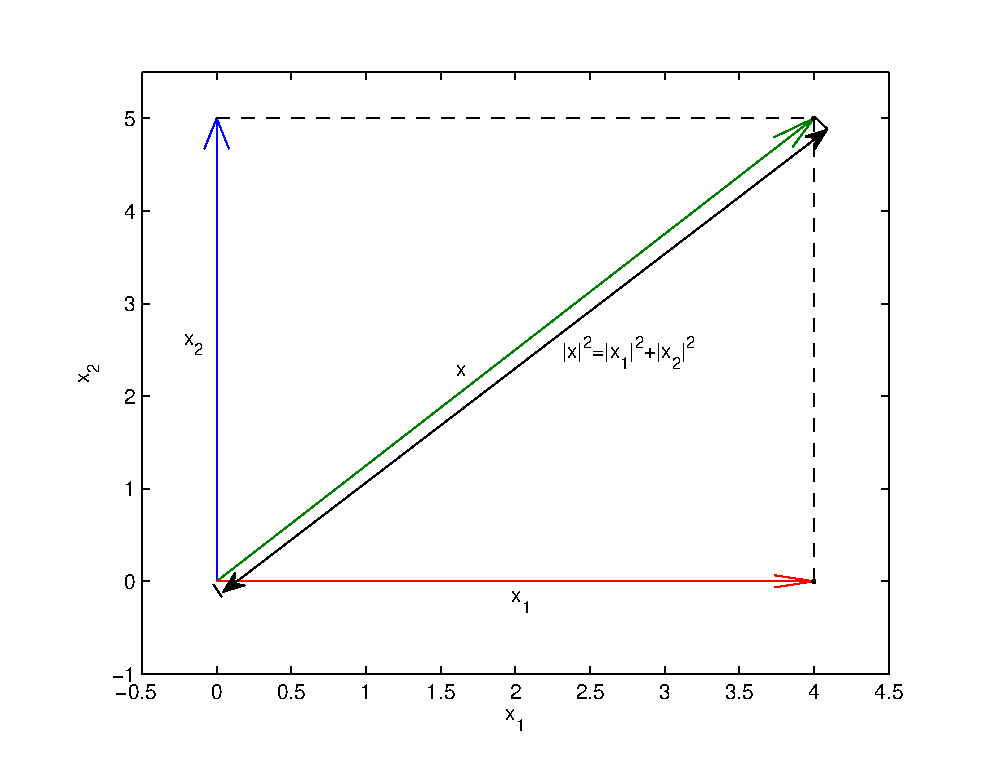
\includegraphics[width=12cm]{pitag.eps}
\caption{interpretación geométrica de la norma de un vector}
\label{fig:pitag}
\end{figure}
\begin{paracol}{2}
A partir de la norma de un vector es posible obtener una expresión alternativa para el producto escalar de dos vectores,
\end{paracol}
\begin{equation*}
a\cdot b=\Vert a \Vert \Vert b \Vert \cos \theta
\end{equation*}
\begin{paracol}{2}
Donde $\theta$ representa el ángulo formado por los dos vectores.
\end{paracol}

\begin{flalign*}
&\mathwitch*_{i=0}^{\infty}\Xi_i(t)&     
\end{flalign*}

\begin{paracol}{2}
Aunque se trate de la manera más común de definir la norma de un vector, la norma 2 no es la única definición posible,

\emph{Norma 1:} Se define como la suma de los valores absolutos de los elementos de un vector,
\end{paracol}
\begin{equation*}
\Vert x \Vert_1 =\vert x_1\vert +\vert x_2 \vert\cdots \vert x_n\vert
\end{equation*}
\begin{paracol}{2}
\emph{Norma p:} Es una generalización de la norma 2,    
\end{paracol}

\begin{equation*}
\Vert x \Vert_p =\sqrt[p]{\vert x_1^p\vert+\vert x_2^p\vert+\cdots \vert x_n^p\vert}=\left( \sum_{i=1}^n\vert x_i^p \vert \right)^\frac{1}{p}
\end{equation*}

\begin{paracol}{2}
\emph{norma $\infty$:} se define como el mayor elemento del vector valor absoluto,    
\end{paracol}

\begin{equation*}
\Vert x \Vert_\infty =max \left\lbrace \vert x_i\vert\right \rbrace 
\end{equation*}

\begin{paracol}{2}
\emph{Norma $-\infty$:} el menor elemento del vector en valor absoluto,
\end{paracol}
\begin{equation*}
\Vert x \Vert_{-\infty} =min \left\lbrace \vert x_i\vert\right \rbrace 
\end{equation*}
\begin{paracol}{2}
En Numpy la norma de un vector puede obtenerse mediante el comando \mintinline{python}{norm(v,p)} La primera variable de entrada debe ser un vector y la segunda el tipo de norma que se desea calcular. Si se omite la segunda variable de entrada, el comando devuelve la norma 2. Para las normas $\infty \text{y} -\infty$ Se emplea el símbolo especial \mintinline{python}{inf} de Numpy. A continuación se incluyen varios ejemplo de utilización,
\end{paracol}

\begin{center}
    \begin{minipage}{.5\textwidth}
        \begin{minted}{python}
In [422]: a
Out[422]: array([1, 2, 3, 4])

In [423]: np.linalg.norm(a,1)
Out[423]: 10.0

In [424]: np.linalg.norm(a,2)
Out[424]: 5.477225575051661

In [425]: np.linalg.norm(a)
Out[425]: 5.477225575051661

In [426]: np.linalg.norm(a,4)
Out[426]: 4.337613136533361

In [427]: np.linalg.norm(a,np.inf)
Out[427]: 4.0

In [428]: np.linalg.norm(a,-np.inf)
Out[428]: 1.0
        \end{minted}
    \end{minipage}
\end{center}

\begin{paracol}{2}
En general, una norma se define como una función de $\mathbb{R}^n \rightarrow \mathbb{R}$, que cumple,
\end{paracol}
\begin{align*}
&\Vert x\Vert \geq 0,\  \Vert x\Vert =0 \Rightarrow x=0\\
&\Vert x+y\Vert \leq \Vert x\Vert +\Vert y\Vert \\
&\Vert \alpha x\Vert = \vert \alpha \vert \Vert x\Vert ,\ \alpha \in \mathbb{R} 
\end{align*}

\begin{flalign*}
&&\reversemathwitch*    
\end{flalign*}

\begin{paracol}{2}
Llamaremos vectores unitarios $u$, a aquellos para los que se cumple que $\Vert u \Vert=1$.

Dos vectores $a$ y $b$ son ortogonales si cumplen que su producto escalar es nulo, $a^Tb=0 \Rightarrow  a\bot b$. Si además ambos vectores tienen módulo unidad, se dice entonces que los vectores son ortonormales.  Desde el punto de vista de su representación geométrica, dos vectores ortogonales, forman entre sí un ángulo recto.

\paragraph{Traza de una matriz.} La traza de una matriz cuadrada , se define como la suma de los elementos que ocupan su diagonal principal,
\end{paracol}
\begin{gather*}
Tr(A)=\sum_{i=1}^na_{ii}\\
Tr\left(
\begin{pmatrix}
1& 4 & 4\\
2& -2 & 2\\
0& 3 & 6
\end{pmatrix}\right)=1-2+6=5
\end{gather*}

\begin{paracol}{2}
La traza de la suma de dos matrices cuadradas $A$ y $B$ del mismo orden, coincide con la suma de las trazas de $A$ y $B$,    
\end{paracol}

\begin{equation*}
tr(A+B)=tr(A)+tr(B)
\end{equation*}

\begin{paracol}{2}
Dada una  matriz $A$ de dimensión $m\times n$  y una matriz $B$ de dimensión $n \times m$, se  cumple que,    
\end{paracol}

\begin{equation*}
tr(AB)=tr(BA)
\end{equation*}
\begin{paracol}{2}
En Python, puede obtenerse directamente el valor de la traza de una matriz $A$, mediante la función \mintinline{python}{np.trace(A)}. En este caso, se trata de un método asociado a cualquier array por lo que tambi.en puede expresarse como \mintinline{python}{A.trace()}  
\end{paracol}

\begin{center}
\begin{minipage}{0.5\textwidth}
\begin{minted}{python}
In [197]: A = np.array([[1,2,3],[3,-2,3],[0,2,-1]])

In [198]: A
Out[198]: 
array([[ 1,  2,  3],
       [ 3, -2,  3],
       [ 0,  2, -1]])

In [199]: np.trace(A)
Out[199]: -2

In [200]: A.trace()
Out[200]: -2
\end{minted}
\end{minipage}
\end{center}


\begin{paracol}{2}
\paragraph{Determinante de una matriz.} 
En Numpy, el determinante de una matriz se calcula  empleando la función \mintinline{python}{det}, del submódulo \mintinline{python}{linalg}. Así, para calcular el determinante de la matriz $A$ del ejemplo anterior,
\end{paracol}
\begin{center}
\begin{minipage}{0.5\textwidth}
\begin{minted}{python}
In [203]: np.linalg.det(A)
Out[203]: 20.000000000000007
\end{minted}
\end{minipage}
\end{center}

\begin{flalign*}
&\mathwitch*_{i=0}^{\infty}\Xi_i(t)&     
\end{flalign*}
\begin{paracol}{2}
El determinante de una matriz $A$, se representa habitualmente como $\vert A \vert$ o, en ocasiones como $det(A)$. Para poder definir el determinante de una matriz, necesitamos antes introducir una serie de conceptos previos. En primer lugar, si consideramos un escalar como una matriz de un solo elemento, el determinante  sería precisamente el valor de ese único elemento,    
\end{paracol}
\begin{equation*}
A=\begin{pmatrix}
a_{11}
\end{pmatrix} \rightarrow \vert A \vert =a_{11}
\end{equation*}
\begin{paracol}{2}
Se denomina menor complementario o simplemente menor, $M_{ij}$ del elemento $a_{ij}$ de una matriz $A$, a la matriz que resulta de eliminar de la matriz $A$ la fila $i$ y la columna $j$ a las que pertenece el elemento $a_{ij}$. Por ejemplo,
\end{paracol}

\begin{align*}
A=\begin{pmatrix}
1& 0& -2\\
3& -2& 3\\
0& 6& 5
\end{pmatrix},& \ 
M_{23}=
\begin{pmatrix}
1& 0\\
0& 6
\end{pmatrix}\\
M_{32}=
\begin{pmatrix}
1& -2\\
3& 3
\end{pmatrix},& \ 
M_{33}=
\begin{pmatrix}
1& 0\\
3& -2
\end{pmatrix}\cdots
\end{align*}

\begin{paracol}{2}
 El  cofactor $C_{ij}$ de un elemento $a_{ij}$ de la matriz $A$, se define a partir del determinante del menor complementario del elemento $a_{ij}$ como,   
\end{paracol}
 
\begin{equation*}
C_{ij}=(-1)^{i+j}\vert M_{ij} \vert
\end{equation*}

\begin{paracol}{2}
Podemos ahora definir el determinante de una matriz $A$ cuadrada de orden $n$, empleando la fórmula de Laplace, 
\end{paracol}
\begin{equation*}
\vert A \vert = \sum_{j=1}^n a_{ij}C_{ij}
\end{equation*}
\begin{paracol}{2}
o alternativamente,
\end{paracol}

\begin{equation*}
\vert A \vert = \sum_{i=1}^n a_{ij}C_{ij}
\end{equation*}
\begin{paracol}{2}
En el primer caso, se dice que se ha desarrollado el determinante a lo largo de la fila $i$. En el segundo caso, se dice que se ha desarrollo el determinante a lo largo de la columna $j$.

 La fórmula de Laplace, obtiene el determinante de una matriz de orden $n\times n$ a partir del cálculo de los determinantes de los menores complementarios de los elementos de una fila; $n$ matrices de orden $(n-1)\times (n-1)$. A su vez, podríamos calcular el determinante de cada menor complementario, aplicando la formula de Laplace y así sucesivamente hasta llegar a matrices de orden $2\times 2$. Para una matriz $2\times 2$, si desarrollamos por la primera fila obtenemos su determinante como,
\end{paracol}

\begin{align*}
A&=\begin{pmatrix}
a_{11}& a_{12}\\
a_{21}& a_{22}
\end{pmatrix}\\
\vert A \vert & =\sum_{j=1}^2a_{1j}C_{1j} =a_{11}C_{11}+a_{12}C_{12}\\
 &=a_{11}(-1)^{1+1}\vert M_{11}\vert +a_{12}(-1)^{1+2}\vert M_{12}\vert \\
 &=-a_{11}a_{22}+a_{12}a_{21}\\
\end{align*}

\begin{paracol}{2}
y si desarrollamos por la segunda columna,
\end{paracol}
\begin{align*}
A&=\begin{pmatrix}
a_{11}& a_{12}\\
a_{21}& a_{22}
\end{pmatrix}\\
\vert A \vert & =\sum_{j=1}^2a_{i2}C_{i2} =a_{12}C_{12}+a_{22}C_{22}\\
 &=a_{12}(-1)^{1+2}\vert M_{12}\vert +a_{22}(-1)^{2+2}\vert M_{22}\vert \\
 &=-a_{12}a_{21}+a_{22}a_{12}\\
\end{align*}

\begin{paracol}{2}
Para una matriz de dimensión arbitraria $n\times n$, el determinante se obtiene aplicando recursivamente la fórmula de Laplace,
\end{paracol}

\begin{align*}
&\vert A  \vert = \sum_{j=1}^na_{ij}C_{ij} =\sum_{j=1}^na_{ij}(-1)^{i+j} \left \vert M_{ij}^{(n-1)\times(n-1)} \right \vert \\
&\left \vert M_{ij}^{(n-1)\times(n-1)} \right \vert = \sum_{k=1}^{n-1}m_{lk}C_{lk} =\sum_{k=1}^{n-1}m_{lk}(-1)^{l+k} \left \vert M_{lk}^{(n-2)\times (n-2)} \right \vert\\
&\vdots \\
&\left \vert M_{st}^{1\times 1}\right \vert=(-1)^{s+t}m_{st} 
\end{align*}
\begin{paracol}{2}
Así, por ejemplo, podemos calcular el determinante de la matriz,
\end{paracol}
\begin{equation*}
A=\begin{pmatrix}
1& 0& -2\\
3& -2& 3\\
0& 6& 5
\end{pmatrix}
\end{equation*}
\begin{paracol}{2}
desarrollándolo por los elementos de la primera columna, como,
\end{paracol}
\begin{align*}
\left\vert A \right\vert =& 1\cdot (-1)^2\cdot 
\left\vert \begin{matrix}
-2& 3\\ 
6& 5
\end{matrix} \right\vert + 3\cdot (-1)^3\cdot
\left\vert \begin{matrix}
0& -2\\ 
6& 5
\end{matrix} \right\vert+ 0\cdot (-1)^4 \cdot 
\left\vert \begin{matrix}
0& -2\\ 
-2& -3
\end{matrix} \right\vert \\
=& 1\cdot (-1)^2\cdot \left[ (-2)\cdot 5 - 6\cdot 3 \right] +3\cdot (-1)^3\cdot  \left[ 0\cdot 5 - 6\cdot (-2)\right] + 0\cdot (-1)^4 \cdot \left[ 0\cdot 3 - (-2)\cdot (-2)\right]= -64
\end{align*}

Podemos programar en Python una función recurrente que calcule el determinante de una matriz de rango $n\times n$. (El método no es especialmente eficiente pero ilustra el uso de funciones recursivas.

\inputminted[
frame=lines,
framesep=2mm,
baselinestretch=1.2,
%bgcolor=LightGray,
label=determinante.py,
fontsize=\footnotesize,
linenos
]{python}{./codigos/Algebra/codigo_abierto/determinante.py}
\begin{flalign*}
&&\reversemathwitch*
\end{flalign*}
\begin{paracol}{2}
Entre las propiedades de los determinantes, destacaremos las siguientes,
\begin{enumerate}
\item El determinante del producto de un escalar $a$ por una matriz $A$ de dimensión $n\times n$ cumple,
\begin{equation*}
\left\vert a\cdot A \right\vert =a^n\cdot \vert A \vert
\end{equation*}
\item El determinante de una matriz es igual al de su traspuesta,
\begin{equation*}
\vert A \vert =\left\vert A^T \right\vert
\end{equation*}

\item El determinante del producto de dos matrices es igual al producto de los determinantes,
\begin{equation*}
\left\vert A_{n\times n} \cdot  B_{n\times n} \right\vert = \left\vert A_{n\times n} \right\vert \cdot \left\vert B_{n\times n} \right\vert 
\end{equation*}
\end{enumerate}

Una matriz es singular si su determinante es cero.

El rango de una matriz se define como el tamaño de la submatriz más grande dentro de $A$, cuyo determinante es distinto de cero. Así por ejemplo la matriz,
\end{paracol}
\begin{equation*}
A=\begin{pmatrix}
1& 2& 3\\
4& 5& 6\\
7& 8& 9
\end{pmatrix} \rightarrow \vert A \vert =0
\end{equation*}
\begin{paracol}{2}
Es una matriz singular y su rango es dos,    
\end{paracol}

\begin{equation*}
\left \vert \begin{matrix}
1& 2\\
4& 5
\end{matrix} \right \vert=-3 \neq 0 \Rightarrow r(A)=2
\end{equation*}
\begin{paracol}{2}
Para una matriz cuadrada no singular, su rango coincide con su dimensión.

En Numpy se puede obtener el rango de una  matriz mediante el comando \mintinline{python}{rank},
\end{paracol}
\begin{center}
\begin{minipage}{0.5\textwidth}
\begin{minted}{python}
In [395]: A
Out[395]: 
array([[1, 2, 3],
       [4, 5, 6],
       [7, 8, 9]])

In [396]: np.linalg.matrix_rank(A)
Out[396]: 2
\end{minted}
\end{minipage}
\end{center}
\begin{paracol}{2}
\paragraph{Inversión.} Dada una matriz cuadrada no singular $A$ de dimension $n$ existe una única matriz $A^{-1}$ de dimension $n$ que cumple,
\begin{equation*}
A\cdot A^{-1}=I_{n\times n}
\end{equation*}
Donde $I_{n\times n}$ es la matriz indentidad de dimensión $n$.
La matriz $A^{-1}$ recibe el nombre de matriz inversa de $A$, y  en numpy puede calcularse a partir de $A$ como \mintinline{python}{np.linalg.inv(A)}, ó \mintinline{python}{np.linalg.matrix_power(A,-1)}
En el segundo caso, estamos empleando la función, del submódulo linalg de numpy, \mintinline{python}{matrix.power(A,n)} que permite calcular el resultado de elevar una matriz a una pontencia $A^n$.
\end{paracol}
\begin{center}
\begin{minipage}{0.7\textwidth}
\begin{minted}{python}
In [409]: B = np.linalg.inv(A)

In [410]: B
Out[410]: 
array([[ 1.29166667, -0.58333333, -0.04166667],
       [ 0.58333333, -0.16666667, -0.08333333],
       [-0.48611111,  0.30555556,  0.06944444]])

In [411]: B @ A
Out[411]: 
array([[ 1.00000000e+00, -5.55111512e-17, -1.11022302e-16],
       [ 0.00000000e+00,  1.00000000e+00, -1.11022302e-16],
       [ 0.00000000e+00,  0.00000000e+00,  1.00000000e+00]])

In [412]: np.linalg.matrix_power(A,-1)
Out[412]: 
array([[ 1.29166667, -0.58333333, -0.04166667],
       [ 0.58333333, -0.16666667, -0.08333333],
       [-0.48611111,  0.30555556,  0.06944444]])
\end{minted}
\end{minipage}
\end{center}
\begin{flalign*}
&\mathwitch*_{i=0}^{\infty}\Xi_i(t)&     
\end{flalign*}
\begin{paracol}{2}
La inversa de una matriz puede obtenerse a partir de la expresión,
\end{paracol}
\begin{equation*}
A^{-1}=\frac{1}{\vert A \vert}[adj(A)]^T
\end{equation*}
\begin{paracol}{2}
Donde $adj(A)$ es la matriz adjunta de $A$, que se obtiene sustituyendo cada elemento $a_{ij}$ de $A$, por su cofactor $C_{ij}$. A continuación incluimos el código en Python de una función, \mintinline{python}{inver}, que calcula la inversa de una matriz. La función \mintinline{python}{inver} llama a su vez a la función \mintinline{python}{dumbdet} descrita más arriba, por lo que debemos importar el módulo \mintinline{python}{determinante} en el módulo en que vamos a crear la función \mintinline{python}{inver}.
\end{paracol}
\inputminted[
frame=lines,
framesep=2mm,
baselinestretch=1.2,
%bgcolor=LightGray,
label=inversa.py,
fontsize=\footnotesize,
linenos
]{python}{./codigos/Algebra/codigo_abierto/inversa.py}

\begin{flalign*}
&&\reversemathwitch*
\end{flalign*}

\begin{paracol}{2}
Algunas propiedades relacionadas con la inversión de matrices son,
\begin{enumerate}
\item Inversa del producto de dos matrices,
\begin{equation*}
(A\cdot B)^{-1}=B^{-1}\cdot A^{-1}
\end{equation*}

\item Determinante de la inversa,
\begin{equation*}
\left\vert A^{-1} \right\vert = \vert A \vert ^{-1}
\end{equation*}

\item Una matriz es ortogonal si su inversa coincide con su transpuesta,
\begin{equation*}
A^{-1}=A^T
\end{equation*}
\end{enumerate}
\end{paracol}

\begin{table}
\bicaption{Algunas funciones matemáticas en Numpy de uso frecuente}{frecuently used mathematical functions included in Numpy}
\label{tabfun}
\begin{tabular}{c|c|c|c}
Tipo&Nombre&variables&función matemática\\
Type&Name&variables&funcion matemática\\
\hline
\hline

Trigonométricas&\multirow{2}{*}{cos}&\multirow{2}{4em}{y=cos(x)}&coseno de un ángulo en radianes\\
Trigonometric& & & Cosine of angle in radians\\
\hline
Trigonometricas&\multirow{2}{*}{sin}&\multirow{2}{4em}{y=sin(x)}&seno de un ángulo en radianes\\
Trigonometric& & &Sine of an angle in radians\\
\hline
Trigonométricas&\multirow{2}{*}{tan}&\multirow{2}{4em}{y=tan(x)}&tangente de un ángulo en radianes\\
Trigonometric & & &Tangent of an angle in radians\\
\hline
Trigonométricas &...&y=arc...(x)&inversa de una función trigonométrica\\
Trigonometric &arcsin&y=arcsin(x)& Inverse of a trigonometric function\\
\hline
\hline
Exponencial&\multirow{2}{*}{exp}&\multirow{2}{*}{y=exp(x)}&\multirow{2}{*}{$e^x$}\\
Exponential& & & \\
\hline
Exponencial&\multirow{2}{*}{log}&\multirow{2}{*}{y=log(x)}&logaritmo natural\\
Exponential & & & Natural logarithm\\
\hline
Exponencial&\multirow{2}{*}{log10}&\multirow{2}{*}{log10(x)}&logaritmo en base 10\\
Exponential& & & Basis 10 logarithm\\
\hline
Exponencial&\multirow{2}{*}{sqrt}&\multirow{2}{*}{y=sqrt(x)}&\multirow{2}{*}{$\sqrt{x}$}\\
Exponential& & & \\
\hline
\hline
Redondeo&\multirow{2}{*}{ceil}&\multirow{2}{*}{y=ceil(x)}& redondeo hacia $+\infty$\\
Rounding& & & rounding towards $+\infty$\\
\hline
Redondeo&\multirow{2}{*}{floor}&\multirow{2}{*}{y=floor(x)}&redondeo hacia $-\infty$\\
Rounding& & & rounding towards $-\infty$ \\
\hline
Redondeo&\multirow{2}{*}{rint}&\multirow{2}{*}{y=rint(x)}&redondeo al entero más próximo\\
Rounding& & & rounding towards the nearest integer\\
\hline
Redondeo&\multirow{2}{*}{fix}&\multirow{2}{*}{y=fix(x)}&redondeo hacia $0$\\
Rounding& & & rounding towards $0$\\
\hline
Redondeo&\multirow{2}{*}{mod}&\multirow{2}{*}{r=mod(x,y)}&resto de la división entera de y entre x\\
Rounding& & & remainder after integer division\\
\hline
\hline
Módulos&\multirow{2}{*}{norm}&\multirow{2}{*}{y=norm(x)}& módulo de un vector x\\
Norms & & & Norm of a vector\\
\hline
Módulos&\multirow{2}{*}{abs}&\multirow{2}{*}{y=abs(x)}&valor absoluto de x\\
Norms & & & Absolute value of x\\
\hline
Módulos&\multirow{2}{*}{sign}&\multirow{2}{*}{y=sign(x)}&función signo; 1 si x $>$ 0, -1 si x $<$ 0, 0 si x=0\\
Norms & & &sign function; 1 if x $>$ 0, -1 if x $<$ 0, 0 if x=0\\ 
\end{tabular}
\end{table}

\begin{paracol}{2}
\subsection{Funciones incluidas en\\ Num\-py.}\index{Funciónes! Funciones incluidas en Numpy} 
Numpy incluye un gran número de funciones. Muchas de ellas  están pensadas para ser aplicadas a arrays o a variables numéricas indistintamente. En el primer caso, la función se aplica elemento a elemento y el resultado es un array con las mismas dimensiones que el original. 

En la tabla \ref{tabfun}, se incluyen algunos ejemplos de las funciones matemáticas más corrientes. No están todas. Para obtener una visión más completa de las funciones disponibles se aconseja acudir a la documntacion de Numpy.
El uso de estas funciones es directo, por ejemplo, el siguiente código calcula la exponencial de los elementos de una matriz,
\end{paracol}

\begin{center}
    \begin{minipage}{0.5\textwidth}
        \begin{minted}{python}
In [1]: import numpy as np

In [2]: A = np.array([[1,2],[2,0],[3,5]])

In [3]: A
Out[3]: 
array([[1, 2],
       [2, 0],
       [3, 5]])

In [4]: np.exp(A)
Out[4]: 
array([[  2.71828183,   7.3890561 ],
       [  7.3890561 ,   1.        ],
       [ 20.08553692, 148.4131591 ]])
        \end{minted}
    \end{minipage}
\end{center}

\begin{paracol}{2}
\section{Operadores vectoriales}\label{opvect}
En esta sección vamos a estudiar el efecto de las operaciones matriciales, descritas en la sección anterior, sobre los vectores. Empecemos por considerar el producto por un escalar $\alpha \cdot a$. El efecto fundamental es modificar el módulo del vector,
\end{paracol}
\begin{equation*}
\alpha \cdot \begin{pmatrix}
a_1\\
a_2\\
a_3
\end{pmatrix}=
\begin{pmatrix}
\alpha a_1\\
\alpha a_2\\
\alpha a_3
\end{pmatrix}\rightarrow \vert \vert \alpha \cdot a \vert \vert =\sqrt{\alpha ^2a_1^2+\alpha ^2a_2^2+\alpha ^2a_3^2}=\vert \alpha \vert  \sqrt{a_1^2+a_2^2+a_3^2}=\vert \alpha \vert \cdot \vert \vert a \vert \vert
\end{equation*}
\begin{paracol}{2}
Gráficamente, si $alpha$ es un número positivo y mayor que la unidad, el resultado del producto será un vector más largo que $a$ con la misma dirección y sentido. Si por el contrario, $\alpha$ es menor que la unidad, el vector resultante será más corto que $a$. Por último si se trata de un número negativo, a los resultados anteriores se añade el cambio de sentido con respecto a $a$. La figura \ref{fig:vmod} muestra gráficamente un ejemplo  del producto de un vector por un escalar.
\end{paracol}
\begin{figure}[h]
\centering
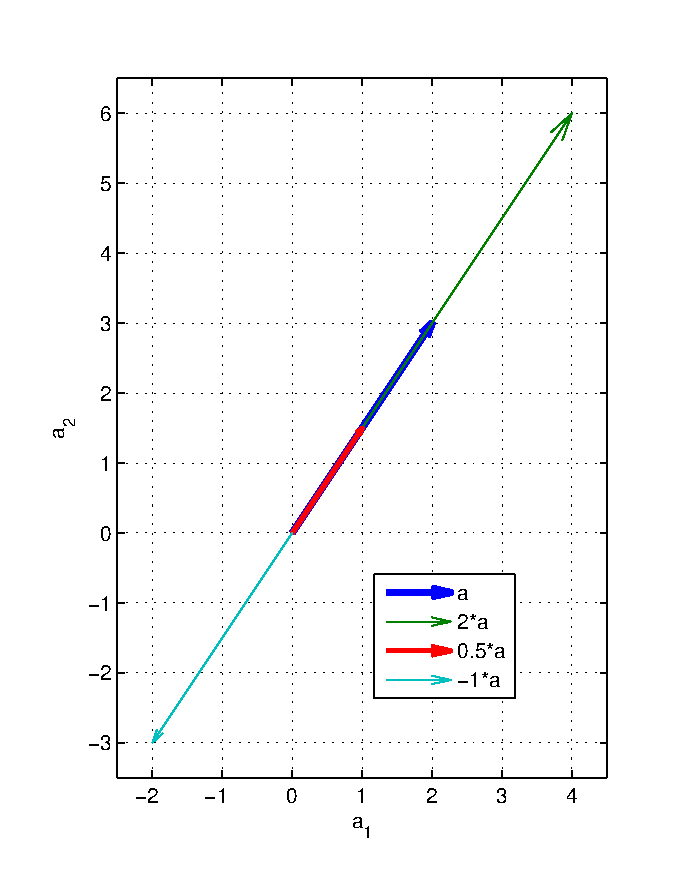
\includegraphics[width=7cm]{vmod.eps}
\caption{efecto del producto de un escalar por un vector}
\label{fig:vmod}
\end{figure}
\begin{paracol}{2}
\paragraph{Combinación lineal.} Combinando la suma de vectores, con el producto por un escalar, podemos generar nuevos vectores, a partir de otros, el proceso se conoce como combinación lineal,
\end{paracol}
\begin{equation*}
c=\alpha \cdot a + \beta \cdot b + \cdots +\theta z
\end{equation*}
\begin{paracol}{2}
Así el vector $c$ sería el resultado de una combinación  lineal de los vectores $a, b \cdots z$. 
Dado un conjunto de vectores, se dice que son linealmente independientes entre sí, si no es posible poner a unos como combinación lineal de otros,
\end{paracol}
\begin{equation*}
\alpha \cdot a + \beta \cdot b + \cdots +\theta z=0 \Rightarrow \alpha =\beta =\cdots =\theta =0
\end{equation*}

\begin{paracol}{2}
Es posible expresar cualquier vector de dimensión $n$ como una combinación lineal de $n$ vectores linealmente independientes.

Supongamos $n=2$, cualquier par de vectores que no estén alineados, pueden generar todos los vectores de dimensión $2$ por ejemplo,
\end{paracol}

\begin{equation*}
\begin{pmatrix}
x_1\\
x_2
\end{pmatrix}=
\alpha \begin{pmatrix}
1\\
2
\end{pmatrix}+\beta \begin{pmatrix}
-1\\
1
\end{pmatrix}
\end{equation*}

La figura \ref{fig:clineal} muestra gráficamente estos dos vectores y algunos de los vectores resultantes de combinarlos linealmente.

\begin{figure}[h]
\centering
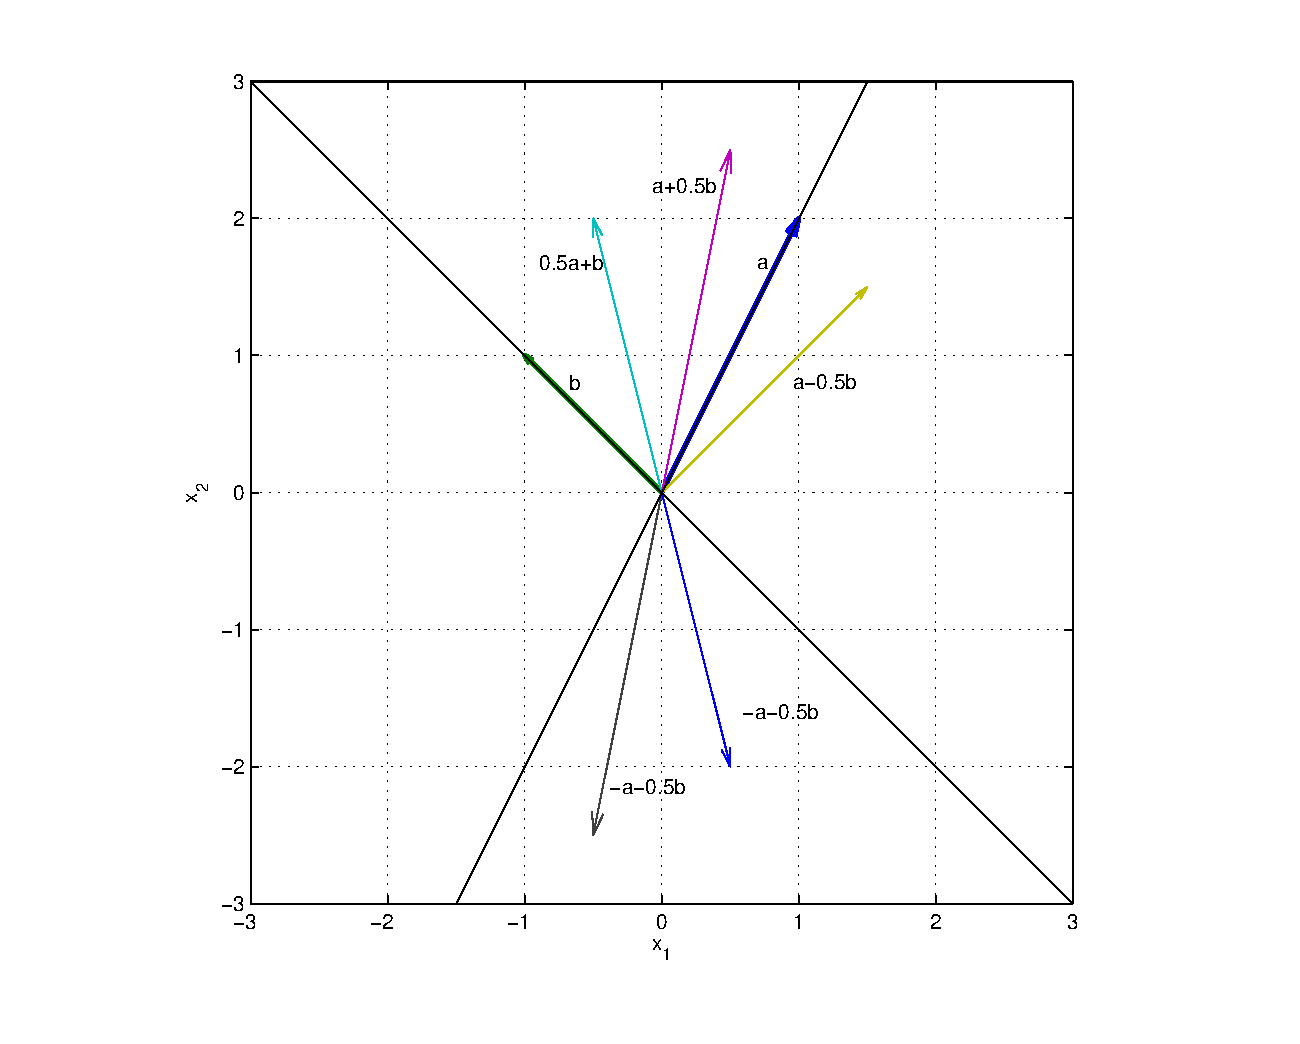
\includegraphics[width=10cm]{clineal.eps}
\caption{Representación gráfica de los vectores $a=(1,2)
$, $b=(-1,1)
$ y algunos vectores, combinación lineal de $a$ y $b$.}
\label{fig:clineal}
\end{figure}
\begin{paracol}{2}
Si tomamos como ejemplo $n=3$, cualquier conjunto de vectores que no estén contenidos en el mismo plano, pueden generar cualquier otro vector de dimensión $3$. Por ejemplo,
\end{paracol}
\begin{equation*}
\begin{pmatrix}
x_1\\
x_2\\
x_3
\end{pmatrix}=\alpha \begin{pmatrix}
1\\
-2\\
1
\end{pmatrix}+ \beta \begin{pmatrix}
2\\
0\\
-1
\end{pmatrix}+ \gamma \begin{pmatrix}
-1\\
1\\
1
\end{pmatrix}
\end{equation*}
\begin{paracol}{2}
La figura \ref{fig:clin3} muestra gráficamente estos tres vectores y el vector resultante de su combinación lineal, con $\alpha=1$, $\beta=-0.5$ y $\gamma=1$.  Es fácil ver a partir de la figura que cualquier otro vector de dimensión $3$ que queramos construir puede obtenerse a partir de los vectores $a$, $b$ y $c$.
\end{paracol}
\begin{figure}[h]
\centering
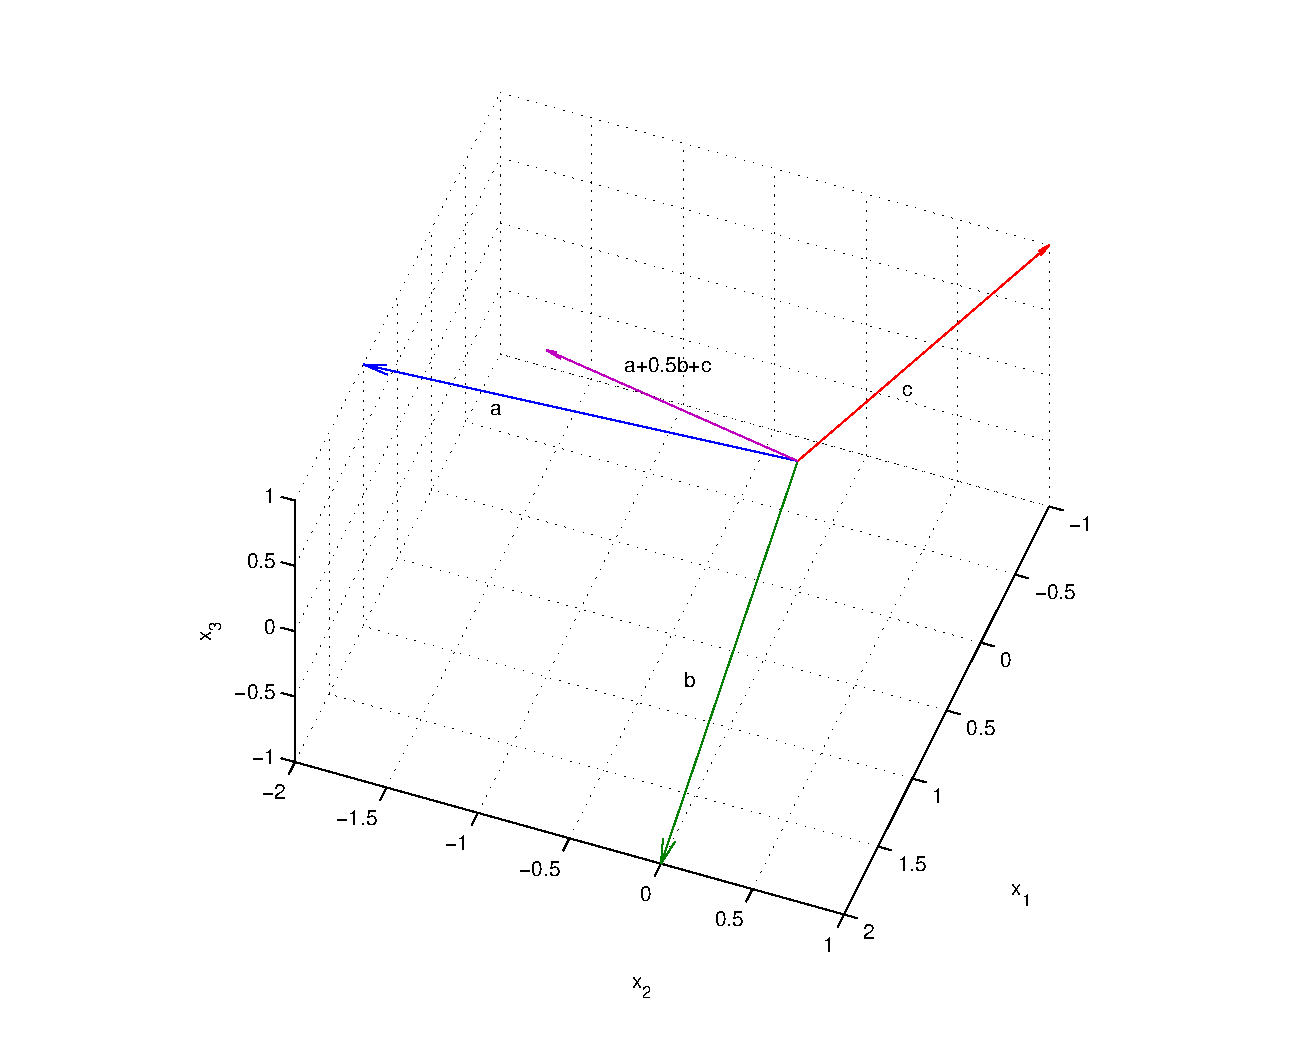
\includegraphics[width=12cm]{clin3.eps}
\caption{Representación gráfica de los vectores $a=(1,-2,1)
$, $b=(2,0,-1)$, $c=(-1,1,1)$ y del vector $a-b+c$.}
\label{fig:clin3}
\end{figure}

\begin{paracol}{2}
\paragraph{Espacio vectorial y  bases del espacio vectorial.} El conjunto de los vectores de dimensión $n$ (matrices de orden $n\times 1$), junto con la suma vectorial y el producto por un escalar, constituye  un  \emph{espacio vectorial} de dimensión $n$.

 Como acabamos de ver, es posible obtener cualquier vector de dicho espacio vectorial a partir de $n$ vectores linealmente independientes del mismo. Un conjunto de $n$ vectores linealmente independientes de un espacio vectorial de dimensión $n$ recibe el nombre de base del espacio vectorial. En principio es posible encontrar infinitas bases distintas para un espacio vectorial de dimensión $n$. Hay algunas particularmente interesantes,
 
 \subparagraph{Bases ortogonales.} Una base ortogonal es aquella en que todos sus vectores son ortogonales entre sí , es decir cumple que su producto escalar es $b^i\cdot b^j=0, i\neq j$. Donde  $b^i$ representa el \emph{i-ésimo} vector de la base, $\mathcal{B}=\left\lbrace b^1, b^2, \cdots, b^n  \right\rbrace $ .
 
 \subparagraph{Bases ortonormales.} Una base ortonormal, es una base ortogonal en la que, además, los vectores de la base tienen módulo $1$. Es decir, $b^i\cdot b^j=0, i\neq j$ y  $b^i\cdot b^j=1, i = j$. Un caso particularmente útil de base ortonormal es la base canónica, formada por los vectores, 
\end{paracol}

\begin{equation*}
\mathcal{C}=\left\lbrace c^1=\begin{pmatrix}
1\\
0\\
0\\
\vdots \\
0
\end{pmatrix}, c^2=\begin{pmatrix}
0\\
1\\
0\\
\vdots \\
0
\end{pmatrix},
\cdots
c^{n-1}=\begin{pmatrix}
0\\
0\\
\vdots \\
1\\
0
\end{pmatrix},
c^n=\begin{pmatrix}
0\\
0\\
\vdots \\
0\\
1
\end{pmatrix} \right\rbrace
\end{equation*} 
\begin{paracol}{2}
Podemos considerar las componentes de cualquier vector como los coeficientes de la combinación lineal de la base canónica que lo representa,
\end{paracol}
\begin{equation*}
a=\begin{pmatrix}
a_1\\
a_2\\
\cdots  \\
a_{n-1}\\
a_n
\end{pmatrix} =a_1\cdot \begin{pmatrix}
1\\
0\\
0\\
\vdots \\
0
\end{pmatrix}+a_2 \cdot  \begin{pmatrix}
0\\
1\\
0\\
\vdots \\
0
\end{pmatrix}+
\cdots +
a_{n-1}\cdot \begin{pmatrix}
0\\
0\\
\vdots \\
1\\
0
\end{pmatrix}+
a_n\cdot \begin{pmatrix}
0\\
0\\
\vdots \\
0\\
1
\end{pmatrix}
\end{equation*}

\begin{paracol}{2}
Por extensión, podemos generalizar este resultado a cualquier otra base, es decir podemos agrupar en un vector los coeficientes de la combinación lineal de los vectores de la base que lo generan. Por ejemplo, si construimos, para los vectores de dimensión $3$ la base,
\end{paracol}

\begin{equation*}
\mathcal{B}=\left\lbrace \begin{pmatrix}
1\\
2\\
0
\end{pmatrix}, \begin{pmatrix}
-1\\
0\\
2
\end{pmatrix}, \begin{pmatrix}
1\\
-1\\
1
\end{pmatrix} \right\rbrace
\end{equation*} 
\begin{paracol}{2}
Podemos entonces representar un vector en la base $\mathcal{B}$ como,
\end{paracol}

\begin{equation*}
\alpha \cdot \begin{pmatrix}
1\\
2\\
0
\end{pmatrix}+\beta \cdot \begin{pmatrix}
-1\\
0\\
2
\end{pmatrix}+ \gamma \cdot \begin{pmatrix}
1\\
-1\\
1
\end{pmatrix} \rightarrow a^{\mathcal{B}}=\begin{pmatrix}
\alpha \\
\beta \\
\gamma
\end{pmatrix}
\end{equation*} 
\begin{paracol}{2}
Donde  estamos empleando el superíndice $^{\mathcal{B}}$, para indicar que las componentes del vector $a$ están definidas con respecto a la base $\mathcal{B}$.

Así por ejemplo el vector,
\end{paracol} 
\begin{equation*}
a^{\mathcal{B}}=\begin{pmatrix}
1.125\\
0.375\\
0.75
\end{pmatrix}
\end{equation*}
\begin{paracol}{2}
Tendría en la base canónica las componentes,
\end{paracol}
\begin{equation*}
a^{\mathcal{B}}=\begin{pmatrix}
1.125\\
0.375\\
0.75
\end{pmatrix} \rightarrow a= 1.125 \cdot \begin{pmatrix}
1\\
2\\
0
\end{pmatrix}+0.375 \cdot \begin{pmatrix}
-1\\
0\\
2
\end{pmatrix}+ 0.75 \cdot \begin{pmatrix}
1\\
-1\\
1
\end{pmatrix} =\begin{pmatrix}
1.5\\
1.5 \\
1.5
\end{pmatrix}
\end{equation*}

\begin{paracol}{2}
La figura \ref{fig:base1}, muestra gráficamente la relación entre los vectores de la base canónica $\mathcal{C}$, los vectores de la base $\mathcal{B}$, y el vector $a$, cuyas componentes se han representado en ambas bases.

Podemos aprovechar el producto de matrices para obtener las componentes en la base canónica $\mathcal{C}$ de un vector representado en una base cualquiera $\mathcal{B}$. Si agrupamos los vectores de la base $\mathcal{B}$, en una matriz $B$,
\end{paracol}
\begin{figure}[h]
\centering
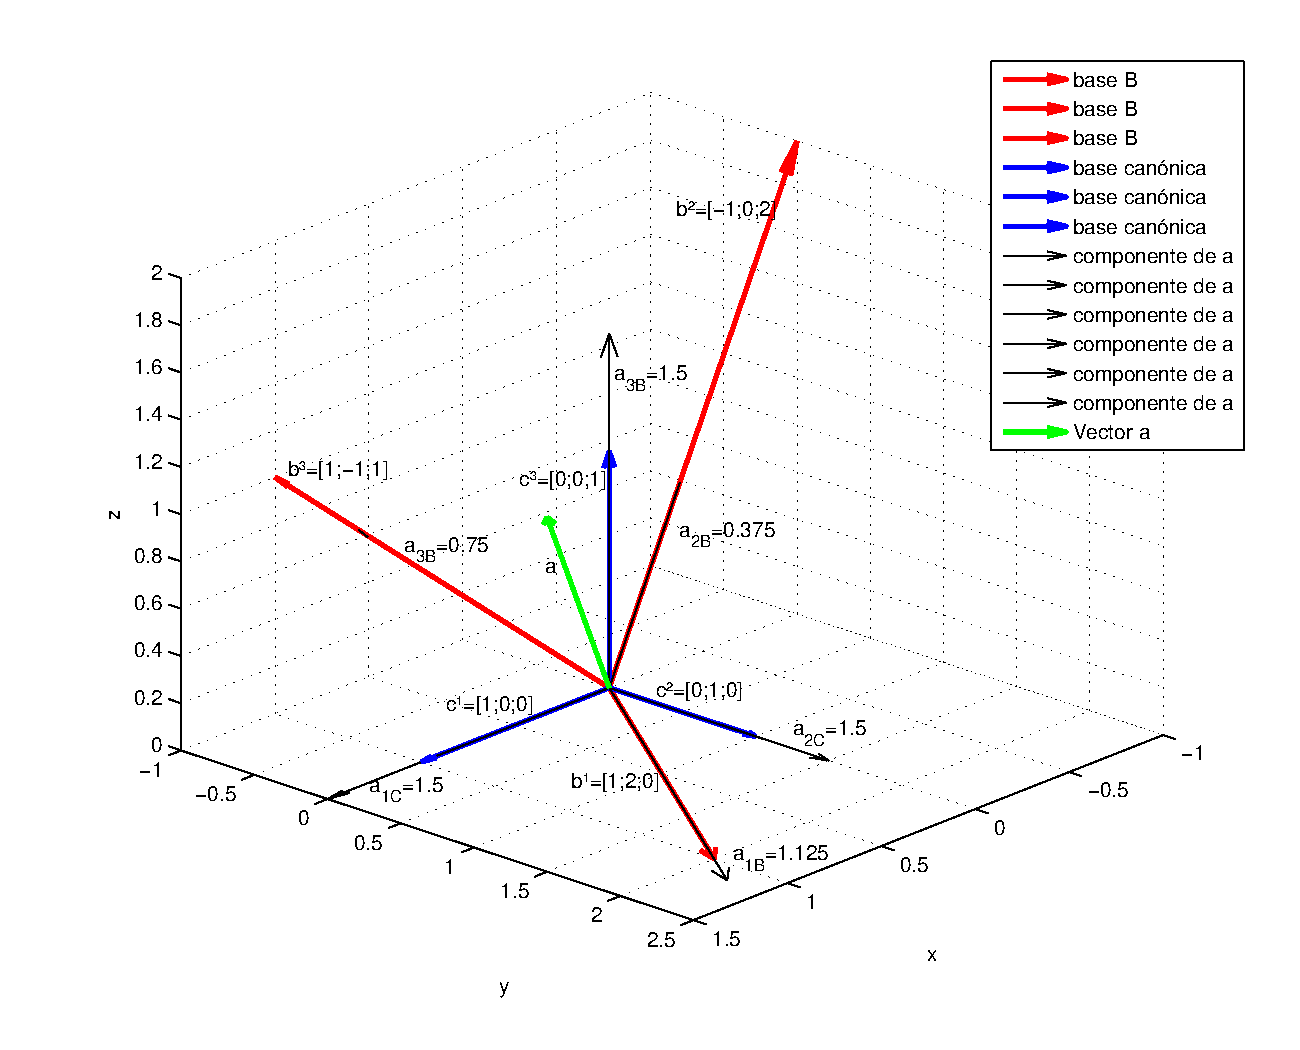
\includegraphics[width=15cm]{base1.eps}
\caption{Representación gráfica del vector $a$, en las base canónica $\mathcal{C}$ y en la base $\mathcal{B}$}
\label{fig:base1}
\end{figure}

\begin{equation*}
\mathcal{B}=\left\lbrace b^1=\begin{pmatrix}
b_{11}\\
b_{21}\\
b_{31}\\
\vdots \\
b_{n1}
\end{pmatrix},b^2=\begin{pmatrix}
b_{12}\\
b_{22}\\
b_{32}\\
\vdots \\
b_{n2}
\end{pmatrix},
\cdots
b^n=\begin{pmatrix}
b_{1n}\\
b_{2n}\\
\vdots \\
b_{(n-1)n}\\
b_{nn}
\end{pmatrix} \right\rbrace \rightarrow
B=\begin{pmatrix}
b_{11}&b_{12}& \cdots & b_{1n}\\
b_{21}&b_{22}& \cdots & b_{2n}\\
b_{31}&b_{32}& \cdots & \vdots \\
\vdots & \vdots & \cdots &  b_{(n-1)n}\\
b_{n1}&b_{n2}& \cdots & b_{nn}\\
\end{pmatrix}
\end{equation*}
\begin{paracol}{2}
Supongamos que tenemos un vector $a$ cuyas componentes en la base $\mathcal{B}$ son,
\end{paracol}

\begin{equation*}
a^{\mathcal{B}}=\begin{pmatrix}
a_1^{\mathcal{B}}\\
a_2^{\mathcal{B}}\\
\vdots \\
a_n^{\mathcal{B}}
\end{pmatrix}
\end{equation*}

\begin{paracol}{2}
Para obtener las componentes en la base canónica, basta entonces multiplicar la matriz $B$, por el vector $a^{\mathcal{B}}$. Así en el ejemplo que acabamos de ver,
\end{paracol}

\begin{equation*}
a=B\cdot a^{\mathcal{B}} \rightarrow a=\begin{pmatrix}
1& -1& 1\\
2& 0& -1\\
0& 2& 1
\end{pmatrix}\cdot \begin{pmatrix}
1.125\\
0.375\\
0.75
\end{pmatrix}
= \begin{pmatrix}
1.5\\
1.5\\
1.5
\end{pmatrix}
\end{equation*}

\begin{paracol}{2}
Por último, una podemos combinar el producto de matrices y la matriz inversa, para obtener las componentes de un vector en una base cualquiera a partir de sus componentes en otra base. Supongamos que tenemos dos bases $\mathcal{B}_1$ y $\mathcal{B}_2$ y un vector $a$. Podemos obtener las componentes de $a$ en la base canónica, a partir de las componentes en la base $\mathcal{B}_1$ como, $a=B_1\cdot a^{\mathcal{B}_1}$ y a partir de sus componentes en la base $\mathcal{B}_2$ como $a=B_2\cdot a^{\mathcal{B}_2}$. Haciendo uso de la matriz inversa,
\end{paracol}

\begin{align*}
a&=B_1\cdot a^{\mathcal{B}_1} \Rightarrow a^{\mathcal{B}_1}=B_1^{-1} \cdot a \\
 a&=B_2\cdot a^{\mathcal{B}_2} \Rightarrow a^{\mathcal{B}_2}=B_2^{-1} \cdot a
\end{align*}

\begin{paracol}{2}
Y sustituyendo obtenemos,
\end{paracol}

\begin{align*}
a^{\mathcal{B}_1}&=B_1^{-1}\cdot B_2 \cdot a^{\mathcal{B}_2}\\
a^{\mathcal{B}_2}&=B_2^{-1} \cdot B_1\cdot a^{\mathcal{B}_1} 
\end{align*}

\begin{paracol}{2}
El siguiente código permite cambiar de base un vector y, si el vector pertenece a $\mathbb{R}^3$, representa gráficamente tanto el vector como las bases antigua y nueva.
\end{paracol}
\inputminted[
frame=lines,
framesep=2mm,
baselinestretch=1.2,
%bgcolor=LightGray,
label=inversa.py,
fontsize=\footnotesize,
linenos
]{python}{./codigos/Algebra/codigo_abierto/cambio_vb.py}

\begin{paracol}{2}
\paragraph{Operadores lineales.} A partir de los visto en las secciones anteriores, sabemos que el producto de una matriz de $A$ de orden $n\times n$  multiplicada por un vector $b$ de dimension $n$ da como resultado un nuevo vector $c=A\cdot b$  de dimensión $n$. Podemos considerar cada matriz $n\times n$ como un \emph{operador lineal}, que transforma unos vectores en otros.  Decimos que se trata de un operador lineal porque las componentes del vector resultante, están relacionadas linealmente con las del vector original, por ejemplo para $n=3$,
\end{paracol}

\begin{equation*}
\begin{pmatrix}
y_1\\
y_2\\
y_3
\end{pmatrix}=\begin{pmatrix}
a_{11}& a_{12}& a_{13}\\
a_{21}& a_{22}& a_{23}\\
a_{31}& a_{32}& a_{33}
\end{pmatrix} \cdot
\begin{pmatrix}
x_1\\
x_2\\
x_3
\end{pmatrix} \rightarrow \begin{matrix}
y_1=a_{11}x_1+a_{12}x_2+a_{13}x_3\\
y_2=a_{21}x_1+a_{22}x_2 +a_{23}x_3\\
y_3=a_{31}x_1+a_{32}x_2+a_{33}x_3
\end{matrix} 
\end{equation*}

\begin{paracol}{2}
Entre los operadores lineales, es posible destacar aquellos que producen transformaciones geométricas sencillas. Veamos algunos ejemplos para vectores bidimensionales,

1. Dilatación: aumenta el módulo de un vector en un factor $\alpha>1$. Contracción: disminuye el módulo de un vector en un factor $0<\alpha<1$. En ambos casos, se conserva la dirección y el sentido del vector original.
\end{paracol} 
\begin{equation*}
R=\begin{pmatrix}
\alpha& 0\\
0& \alpha
\end{pmatrix} \rightarrow R\cdot a = \begin{pmatrix}
\alpha& 0\\
0& \alpha
\end{pmatrix} \cdot \begin{pmatrix}
a_1\\
a_2
\end{pmatrix}= \begin{pmatrix}
\alpha \cdot a_1\\
\alpha \cdot a_2
\end{pmatrix}
\end{equation*}
\begin{paracol}{2}
2. Reflexión de un vector respecto al eje x, conservando su módulo,
\end{paracol}
\begin{equation*}
R_x=\begin{pmatrix}
1& 0\\
0& -1
\end{pmatrix} \rightarrow R_x\cdot a = \begin{pmatrix}
1& 0\\
0& -1
\end{pmatrix} \cdot \begin{pmatrix}
a_1\\
a_2
\end{pmatrix}= \begin{pmatrix}
a_1\\
-a_2
\end{pmatrix}
\end{equation*}
\begin{paracol}{2}
3. Reflexión de un vector respecto al eje y, conservando su módulo,
\end{paracol}
\begin{equation*}
R_y=\begin{pmatrix}
-1& 0\\
0& 1
\end{pmatrix} \rightarrow R_y\cdot a = \begin{pmatrix}
-1& 0\\
0& 1
\end{pmatrix} \cdot \begin{pmatrix}
a_1\\
a_2
\end{pmatrix}= \begin{pmatrix}
-a_1\\
a_2
\end{pmatrix}
\end{equation*}
\begin{paracol}{2}
4. Reflexión respecto al origen: Invierte el sentido de un vector, conservando su módulo y dirección,
\end{paracol}
\begin{equation*}
R=\begin{pmatrix}
-1& 0\\
0& -1
\end{pmatrix} \rightarrow R\cdot a = \begin{pmatrix}
-1& 0\\
0& -1
\end{pmatrix} \cdot \begin{pmatrix}
a_1\\
a_2
\end{pmatrix}= \begin{pmatrix}
-a_1\\
-a_2
\end{pmatrix}
\end{equation*}
\begin{paracol}{2}
5. Sería equivalente a aplicar una reflexión respecto al eje x y luego respecto al eje y o viceversa,
\end{paracol}
$R=R_x\cdot R_y= R_y\cdot R_x$.
\begin{paracol}{2}
 Rotación en torno al origen un ángulo $\theta$,
\end{paracol}
\begin{equation*}
R_{\theta}=\begin{pmatrix}
cos(\theta)& -sin(\theta)\\
sin(\theta)& cos(\theta)
\end{pmatrix} \rightarrow R_{\theta}\cdot a = \begin{pmatrix}
cos(\theta)& -sin(\theta)\\
sin(\theta)& cos(\theta)
\end{pmatrix} \cdot \begin{pmatrix}
a_1\\
a_2
\end{pmatrix}= \begin{pmatrix}
a_1cos(\theta)-a_2sin(\theta)\\
a_1sin(\theta)+a_2cos(\theta)
\end{pmatrix}
\end{equation*}


La figura \ref{fig:ltrans} muestra los vectores resultantes de aplicar las transformaciones lineales que acabamos de describir al vector,  $ a=\bigl( \begin{smallmatrix}
1\\
2
\end{smallmatrix} \bigr)$,

\begin{figure}[h]
\centering
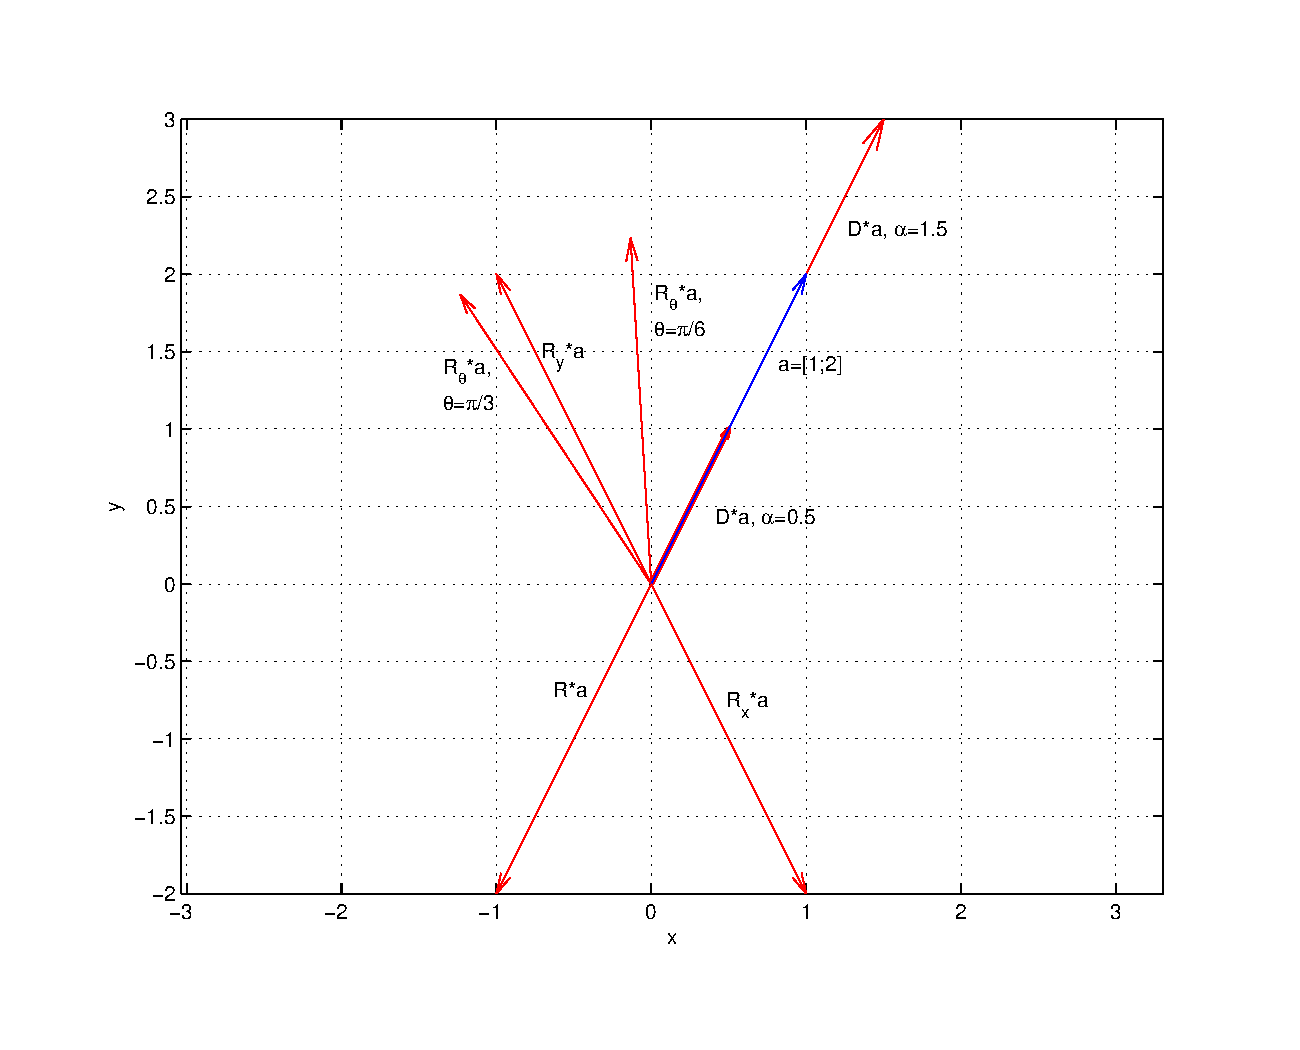
\includegraphics[width=12cm]{ltrans.eps}
\caption{Transformaciones lineales del vector $a=[1;2]$. $D$, dilatación/contracción en un factor $1.5$/$0.5$. $R_x$, reflexión respecto al eje x. $R_y$, reflexión respecto al eje y. $R_{\theta}$ rotaciones respecto al origen para ángulos $\theta=\pi /6$ y $\theta=\pi /3$}
\label{fig:ltrans}
\end{figure}

\begin{paracol}{2}
\paragraph{Norma de una matriz.} La norma de una matriz se puede definir a partir del efecto que produce al actuar, como un operador lineal, sobre un vector. En este caso, se les llama normas \emph{inducidas}. Para una matriz $A$ de orden $m\times n$, $y_{(m)}=A_{(m\times n)}x_{(n)}$, La norma inducida de $A$ se define en función de las normas de los vectores $x$ de su dominio y de las normas de los vectores $y$ de su rango como,
\end{paracol}
\begin{equation*}
\Vert A \Vert =\max_{x \neq 0} \frac{\Vert y \Vert}{\Vert x \Vert}=\max_{x \neq 0} \frac{\Vert Ax \Vert}{\Vert x \Vert}
\end{equation*}

\begin{paracol}{2}
Se puede interpretar como el factor máximo con que el que la matriz $A$ puede \emph{alargar} un vector cualquiera. Es posible definir la norma inducida en función de los vectores unitarios del dominio,
\end{paracol}
\begin{equation*}
\Vert A \Vert =\max_{x \neq 0} \frac{\Vert Ax \Vert}{\Vert x \Vert}= \max_{x \neq 0} \left\Vert A\frac{x}{\Vert x \Vert} \right\Vert= \max_{\Vert x \Vert =1}\Vert Ax \Vert
\end{equation*}

\begin{paracol}{2}
Junto a la norma inducida que acabamos de ver, se definen las siguientes normas,

1. Norma 1: Se suman los elementos de cada columna de la matriz, y se toma como norma el valor máximo de dichas sumas,
\end{paracol}
\begin{equation*}
\Vert A_{m,n} \Vert _{1} = \max_j \sum_{i=1}^m a_{ij}
\end{equation*}
\begin{paracol}{2}
2. Norma $\infty$: Se suman los elementos de cada fila y se toma como norma $\infty$ el valor máximo de dichas sumas.
\end{paracol}
\begin{equation*}
\Vert A_{m,n} \Vert _{\infty} = \max_i \sum_{j=1}^m a_{ij}
\end{equation*}
\begin{paracol}{2}
3. Norma 2: Se define como el mayor de los valores singulares de una matriz. (Ver sección 
\end{paracol}
\ref{sec:SVD}).
\begin{equation*}
\Vert A_{m,n} \Vert _2 = \sigma_{1}
\end{equation*}
\begin{paracol}{2}
4. Norma de Frobenius. Se define como la raíz cuadrada de la suma de los cuadrados de todos los elementos de la matriz,
\end{paracol}
\begin{equation*}
\Vert A_{m,n} \Vert _F =\sqrt{\sum_{i=1}^m \sum_{j=1}^m a_{ij}^2}
\end{equation*}
\begin{paracol}{2}
Que también puede expresarse de forma mas directa como,
\end{paracol}
\begin{equation*}
\Vert A_{m,n} \Vert _F =\sqrt{tr(A^T\cdot A)}
\end{equation*}
\begin{paracol}{2}
En Numpy, es posible calcular las distintas normas de una matriz, de modo análogo a como se calculan para el caso de vectores,  mediante el comando \texttt{norm(A,p)}. Donde \texttt{A}, es ahora un a matriz y \texttt{p} especifica el tipo de norma que se quiere calcular. En el caso de una matriz, el parámetro \texttt{p} solo puede tomar los valores, \texttt{1} (norma 1), \texttt{2} (norma 2), \texttt{inf} (norma $\infty$), y \texttt{'fro'} (norma de frobenius). Esta última es la norma por defecto, y es la que se optiene si se no se define el tipo de normar. El siguiente ejemplo muestra el cálculo de las normas 1, 2, $\infty$ y de Frobenius de la misma matriz.
\end{paracol}
\begin{center}
    \begin{minipage}{0.5\textwidth}
    \begin{minted}{python}
In [11]: A = np.array([[1,-1,3],[2,0,-2],[3,1,2]])

In [12]: A
Out[12]: 
array([[ 1, -1,  3],
       [ 2,  0, -2],
       [ 3,  1,  2]])

In [13]: np.linalg.norm(A)
Out[13]: 5.744562646538029

In [14]: np.linalg.norm(A,'fro')
Out[14]: 5.744562646538029

In [15]: np.linalg.norm(A,1)
Out[15]: 7.0

In [17]: np.linalg.norm(A,inf)
Out[17]: 6.0

In [18]: np.linalg.norm(A,2)
Out[18]: 4.552861506620628
\end{minted}
\end{minipage}
\end{center}

\begin{paracol}{2}
\paragraph{Formas cuadráticas.} Se define como forma cuadrática a la siguiente operación entre una matriz cuadrada $A$ de orden $n \times n$ y un vector $x$ de dimensión $n$,
\end{paracol}
\begin{equation*}
\alpha=x^T\cdot A \cdot x, \ \alpha \in \mathbb{R}
\end{equation*}

\begin{paracol}{2}
El resultado es un escalar. Así por ejemplo,
\end{paracol}

\begin{equation*}
A=\begin{pmatrix}
1& 2& -1\\
2& 0& 2\\
3& 2& -2
\end{pmatrix}, \ x=\begin{pmatrix}
1\\
2\\
3
\end{pmatrix} \rightarrow \begin{pmatrix}
1& 2& 3
\end{pmatrix} \cdot \begin{pmatrix}
1& 2& -1\\
2& 0& 2\\
3& 2& -2
\end{pmatrix} \cdot \begin{pmatrix}
1\\
2\\
3
\end{pmatrix}= 21
\end{equation*}
\begin{paracol}{2}
Para dimensión $n=2$,
\end{paracol}
\begin{equation*}
\alpha =\begin{pmatrix}
x_1& x_2
\end{pmatrix}\cdot \begin{pmatrix}
a_{11}& a_{12}\\
a_{21}& a_{22}
\end{pmatrix}\cdot \begin{pmatrix}
x_1\\
x_2
\end{pmatrix} \rightarrow x_3\equiv \alpha=a_{11}x_1^2+(a_{12}+a_{21})x_1x_2+a_{22}x_2^2
\end{equation*}

\begin{paracol}{2}
Lo que obtenemos, dependiendo de los signos de $a_{11}$ y $a_{12}$, es la ecuación de un paraboloide o un hiperboloide. En la figura \ref{fig:parabol} Se muestra un ejemplo,
\end{paracol}
\begin{figure}[h]
\centering
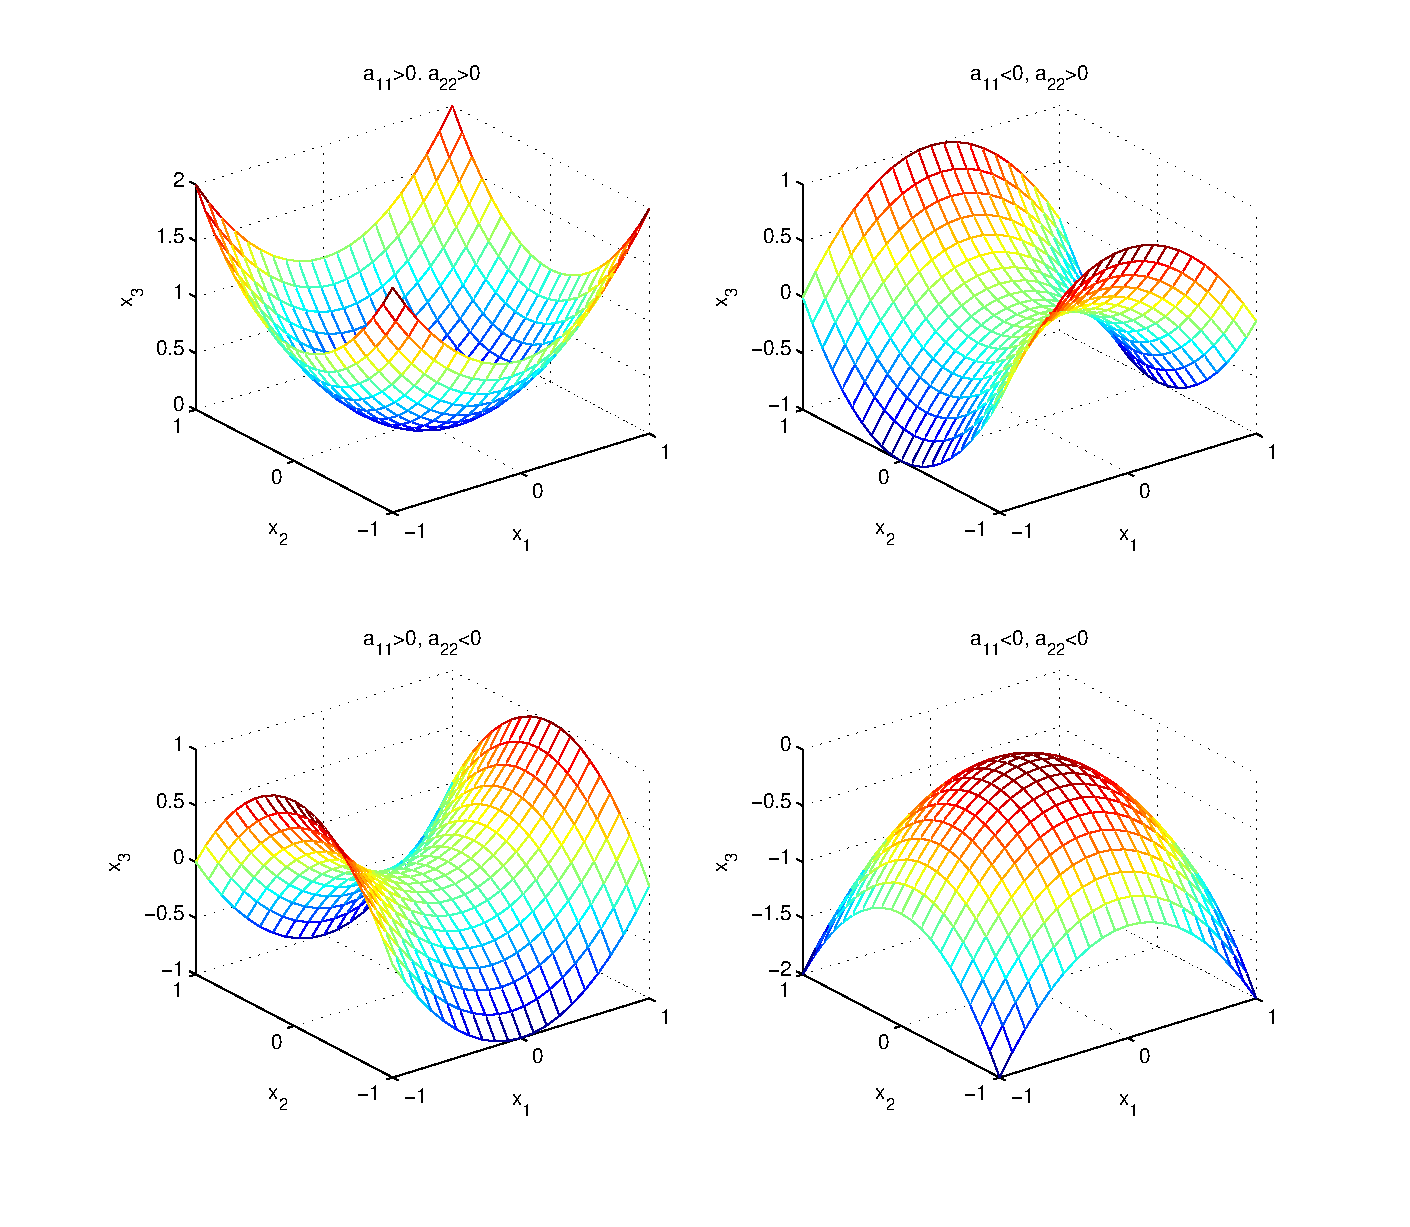
\includegraphics[width=14cm]{parabol.eps}
\caption{Formas cuadráticas asociadas a las cuatro matrices diagonales: $\vert a_{11}\vert=\vert a_{22}\vert=1$, $a_{12}=a_{21}=0$}
\label{fig:parabol}
\end{figure}
\begin{paracol}{2}
Veamos brevemente, algunas propiedades relacionadas con  las formas cuadráticas,

1. Una matriz $A$ de orden $ n\times n$ se dice que es definida positiva si da lugar a una forma cuadrática que es siempre mayor que cero para cualquier vector no nulo,
\end{paracol}
\begin{equation*}
x^T \cdot A \cdot x > 0, \forall x \neq 0 
\end{equation*}
\begin{paracol}{2}
2. Una matriz \emph{simétrica} es definida positiva si todos sus \emph{valores propios} (ver sección \ref{sec:diag}) son positivos.

3. Una matriz no simétrica $A$ es definida positiva si su parte simétrica $A_s=(A+A^T)/2$ lo es.
\end{paracol}
\begin{equation*}
x\cdot A_s\cdot >0, \forall x \neq 0 \Rightarrow x\cdot A\cdot >0, \forall x \neq 0
\end{equation*}

\begin{flalign*}
&&\reversemathwitch*
\end{flalign*}

\begin{paracol}{2}
\section{Tipos de matrices empleados frecuentemente}\label{tiposm}
Definimos a continuación algunos tipos de matrices frecuentemente empleados en álgebra, algunos ya han sido introducidos en secciones anteriores. Los reunimos todos aquí para facilitar su consulta

1 Matriz ortogonal: Una matriz $A_{n\times n}$ es ortogonal cuando su inversa coincide con su traspuesta.
\end{paracol}
\begin{equation*}
A^T=A^{-1}
\end{equation*}
\begin{paracol}{2}
ejemplo,
\end{paracol}

\begin{equation*}
A=\begin{pmatrix}
1/3& 2/3& 2/3\\
2/3& -2/3& 1/3\\
2/3& 1/3& -2/3\\
\end{pmatrix} \rightarrow A\cdot A^T =A^T\cdot A= \begin{pmatrix}
1& 0& 0\\
0& 1& 0\\
0& 0& 1
\end{pmatrix}
\end{equation*}
\begin{paracol}{2}
2. Matriz simétrica: Una matriz $A_{n\times n}$ es simétrica cuando es igual que su traspuesta,
\end{paracol}
\begin{equation*}
A=A^T \rightarrow a_{ij}=a_{ji}
\end{equation*}
\begin{paracol}{2}
ejemplo,
\end{paracol}
\begin{equation*}
A=\begin{pmatrix}
1& -2& 3\\
-2& 4& 0\\
3& 0& -5
\end{pmatrix}
\end{equation*}
\begin{paracol}{2}
3. Matriz Diagonal: Una matriz $A$  es diagonal si solo son distintos de ceros los elementos de su diagonal principal,
\end{paracol}

\begin{equation*}
\begin{pmatrix}
a_{11}& 0& \cdots & 0\\
0& a_{22}& \cdots & 0\\
\vdots & \vdots & \ddots & 0\\
0& 0& \cdots & a_{nn}
\end{pmatrix} \rightarrow
a_{ij}=0,\ \forall i\neq j
\end{equation*}

\begin{paracol}{2}
4. Matriz triangular superior: Una matriz es triangular superior cuando todos los elementos situados por debajo de la diagonal son cero. Es estrictamente diagonal superior si además los elementos de la diagonal también son cero,
\end{paracol}
\begin{align*}
TRS& \rightarrow a_{ij} = 0, \ \forall i\geq j \\
ETRS& \rightarrow a_{ij} = 0, \ \forall i > j 
\end{align*}
\begin{paracol}{2}
ejemplos,
\end{paracol}

\begin{align*}
TRS&=\begin{pmatrix}
1 & 3 & 7\\
0 & 2 & -1\\
0 & 0 & 4
\end{pmatrix}\\
ETRS&=\begin{pmatrix}
0 & 3 & 7\\
0 & 0 & -1\\
0 & 0 & 0
\end{pmatrix}\\
\end{align*}
\begin{paracol}{2}
5. Matriz triangular inferior: Una matriz es triangular inferior si todos los elementos pro encima de su diagonal son cero. Es estrictamente triangular inferior si además los elementos de su diagonal son también cero,
\end{paracol}
\begin{align*}
TRI& \rightarrow a_{ij} = 0, \ \forall i\leq j \\
ETRI& \rightarrow a_{ij} = 0, \ \forall i < j 
\end{align*}
\begin{paracol}{2}
ejemplos,
\end{paracol}

\begin{align*}
TRI&=\begin{pmatrix}
1 & 0 & 0\\
3 & 2 & 0\\
7 & -1 & 4
\end{pmatrix}\\
ETRI&=\begin{pmatrix}
0 & 0 & 0\\
3 & 0 & 0\\
7 & -1 & 0
\end{pmatrix}\\
\end{align*}
\begin{paracol}{2}
6. Matriz definida Positiva. Una Matriz $A_{n \times n}$ es definida positiva si dado un vector $x$ no nulo cumple,
\end{paracol}
\begin{equation*}
x^T\cdot A \cdot x > 0, \ \forall x\neq 0
\end{equation*}
si,
\begin{equation*}
x^T\cdot A \cdot x \geq 0, \ \forall x\neq 0
\end{equation*}
\begin{paracol}{2}
entonces la matriz $A$ es semidefinida positiva.

7. Una matriz es Diagonal dominante si cada uno de los elementos de la diagonal en valor absoluto es mayor que la suma de los valores absolutos de los elementos de la fila a la  que pertenece.
\end{paracol}

\begin{equation*}
\lvert a_{ii} \rvert > \sum_{j\neq i} \lvert a_{ij} \rvert, \ \forall i
\end{equation*}
\begin{paracol}{2}
ejemplo,
\end{paracol}
\begin{equation*}
A=\begin{pmatrix}
10& 2 & 3\\
2& -5 & 1\\
4& -2 & 8
\end{pmatrix}\rightarrow \left\{ \begin{aligned}
10& > 2+3\\
5&> 2+1\\
8& > 4+2
\end{aligned} \right. 
\end{equation*}

\begin{paracol}{2}
\section{Factorización de matrices}\label{sec:fact}
La factorización de matrices, consiste en la descomposición de una matriz en el producto de dos o más matrices. Las matrices resultantes de la factorización se eligen de modo que simplifiquen, o hagan más robustas numéricamente determinadas operaciones matriciales: Cálculos de determinantes, inversas, etc. A continuación se describen las más comunes.

\subsection{Factorizacion LU}\label{sec:LU}
Consiste en factorizar una matriz como el producto de una matriz triangular inferior $L$ por una  matriz triangular superior $U$, $A=L\cdot U$. Por ejemplo,
\end{paracol}
\begin{equation*}
\begin{pmatrix}
3& 4& 2\\
2& 0& 1\\
3& 2& 1
\end{pmatrix} = \begin{pmatrix}
1& 0& 0\\
^2/_3 & 1& 0\\
1& ^3/_4& 1
\end{pmatrix}\cdot \begin{pmatrix}
3& 4& 2\\
0& ^{-8}/_3& ^{-1}/_3\\
0& 0& ^{-3}/_4
\end{pmatrix}
\end{equation*}
\begin{paracol}{2}
Una aplicación inmediata, es el calculo del determinante. Puesto que el determinante de una matriz triangular, es directamente el producto de los elementos de la diagonal.

En el ejemplo anterior,
\end{paracol}
\begin{equation*}
\vert A \vert = 6 \equiv \vert L \vert\cdot\vert U\vert =1 \cdot 1 \cdot 1 \cdot 3 \cdot (-\frac{8}{3})\cdot (-\frac{3}{4})=6    
\end{equation*}


% Hasta ahora, hemos descrito un procedimiento para transformar una matriz cualquiera en una matriz triangular superior. Nuestro objetivo era obtener la descomposición de un matriz en el producto de dos,  una triangular inferior y otra triangular superior.  En primer lugar, podemos asociar    el procedimiento descrito de eliminación gaussiana al producto de matrices. Volviendo al ejemplo anterior, si construimos la matriz $\lambda_1$
% \begin{equation*}
% \lambda_1=\begin{pmatrix} 
% 1& 0& 0& 0\\
% -2/3& 1& 0& 0\\
% -3/3& 0& 1& 0\\
% -5/3& 0& 0& 1
% \end{pmatrix}
% \end{equation*},
% El producto $\lambda_1 \cdot A$ da como resultado la matriz,

% \begin{equation*} 
%  U_1=\begin{pmatrix}
% 3& 4& 2&5\\
% 0& -2.66& -0.33& -5.33\\
% 0& -2& -1& -3\\
% 0& -4.66& -0.33& -6.33
% \end{pmatrix}=\begin{pmatrix} 
% 1& 0& 0& 0\\
% -2/3& 1& 0& 0\\
% -3/3& 0& 1& 0\\
% -5/3& 0& 0& 1
% \end{pmatrix}\cdot \begin{pmatrix}
% 3& 4& 2&5\\
% 2& 0& 1& -2\\
% 3& 2& 1& 8\\
% 5& 2& 3& 2
% \end{pmatrix}
% \end{equation*}

% De modo análogo, $U_2=\lambda_2 \cdot U_1$
 
% \begin{equation*}
% \lambda_2=\begin{pmatrix} 
% 1& 0& 0& 0\\
% 0& 1& 0& 0\\
% 0& -2/2.66& 1& 0\\
% 0& -4.66/2.66& 0& 1
% \end{pmatrix}
% \end{equation*}

% \begin{equation*}
% U_2= \begin{pmatrix}
% 3& 4& 2&5\\
% 0& -2.6& -0.33& -5.33\\
% 0& 0& -0.75& 7\\
% 0& 0& 0.25& 3
% \end{pmatrix}
% \end{equation*}

% Por último, $U=\lambda_3 \cdot U_2$

% \begin{equation*}
%  \lambda_3 =\begin{pmatrix}
% 1& 0& 0&0\\
% 0& 1& 0& 0\\
% 0& 0& 1& 0\\
% 0& 0& 0.25/0.75 & 1
% \end{pmatrix}
% \end{equation*}

% \begin{equation*}
%  U =\begin{pmatrix}
% 3& 4& 2&5\\
% 0& -2.66& -0.33& -5.33\\
% 0& 0& -0.75& 7\\
% 0& 0& 0& 5.33
% \end{pmatrix}
% \end{equation*}

% De nuevo, podemos generalizar el procedimiento empleado; cada matriz $\lambda_j$ \emph{elimina} todos los elementos de la columna $n$ de una matriz $A$ , situados por debajo de la diagonal. La  matriz $\lambda_j$  toma la forma general,

% \begin{equation*}
% \lambda_j=\begin{pmatrix}
% 1& \cdots & 0& 0& 0& \cdots & 0\\
%  \vdots &  &  \vdots & \vdots &  \vdots & & \vdots\\
% 0& \cdots & 1& 0& 0& \cdots & 0\\
% 0& \cdots & 0& 1& 0& \cdots & 0\\
% 0& \cdots &0 & -a_{j+1,j}/a_{jj}& 0& \cdots & 0\\
% 0& \cdots &0 & -a_{j+2,j}/a_{jj}& 1& \cdots & 0\\
%  \vdots &  &  \vdots & \vdots &  \vdots & & \vdots\\
% 0& \cdots & 0& -a_{n,j}/a_{jj}& 0&\cdots & 1\\
% \end{pmatrix}
% \end{equation*} 
% Solo los elementos de la diagonal, que toman el valor $1$, y los elementos de la columna $j$ situados por debajo de la diagonal son distintos de cero.

% A partir de la definición de las matrices $\lambda_j$, podemos obtener una relación entre la matriz triangular superior $U$  obtenida al final del proceso de eliminación, y la matriz inicial $A$ de orden $n\times n$ para ello, en cada paso multiplicamos tanto por $\lambda_j$ como por su inversa $\lambda_j^{-1}$,
% \begin{align*}
% A&=\lambda_1^{-1}\cdot \overbrace{\lambda_1\cdot A}^{U_1}\\
% A&=\lambda_1^{-1}\cdot\lambda_2^{-1} \cdot \overbrace{\lambda_2  \cdot \lambda_1 A}^{U_2}\\
% A&=\lambda_1^{-1}\cdot \lambda_2^{-1}\cdot \overbrace{ \lambda_3^{-1}\cdot  \lambda_3 \cdot  \lambda_2\cdot \lambda_1 \cdot A}^{U_3}\\
% \vdots \\
% A&=\lambda_1^{-1} \cdot  \lambda_2^{-1}\cdot  \lambda_3^{-1} \cdots  \lambda_n ^{-1}\cdot \overbrace{\lambda_n \cdots \lambda_3 \cdot \lambda_2\cdot \lambda_1  \cdot A}^{U}
% \end{align*}

% Las matrices $\lambda_j^{-1}$ tienen dos propiedades que las hacen particularmente fáciles de manejar:  la primera es que cumplen que  su inversa  $\lambda_j^{-1}$ puede obtenerse a partir de $\lambda_j$, sin más que cambiar de signo los elementos distintos de cero que no pertenecen a la diagonal (Compruébalo),
% \begin{equation*}
%  \lambda_j^{-1}=\begin{pmatrix}
% 1& \cdots & 0& 0& 0& \cdots & 0\\
%  \vdots &  &  \vdots & \vdots &  \vdots & & \vdots\\
% 0& \cdots & 1& 0& 0& \cdots & 0\\
% 0& \cdots & 0& 1& 0& \cdots & 0\\
% 0& \cdots &0 & a_{j+1j}/a_{jj}& 0& \cdots & 0\\
% 0& \cdots &0 & a_{j+2j}/a_{jj}& 1& \cdots & 0\\
%  \vdots &  &  \vdots & \vdots &  \vdots & & \vdots\\
% 0& \cdots & 0& a_{nj}/a_{jj}& 0&\cdots & 1\\
% \end{pmatrix}
% \end{equation*}

% La segunda propiedad es que el producto $L=\lambda_1^{-1} \cdot  \lambda_2^{-1}\cdot  \lambda_3^{-1} \cdots  \lambda_n ^{-1}$, se puede obtener progresivamente, a la vez que se construye $U$, sin más que ir juntando en una única matriz $L$ las columnas de $\lambda_1^{-1}$, $\lambda_2^{-1}$, etc. que contienen elementos no nulos, en nuestro ejemplo,
% \begin{equation*}
%  L =\begin{pmatrix}
% 1& 0& 0&0\\
% 2/3& 1& 0& 0\\
% 3/3& 2/2.66& 1& 0\\
% 5/3& 4.66/2.66& -0.25/0.75 & 1
% \end{pmatrix}
% \end{equation*}

% y, en general,

% \begin{equation*}
%  L=\begin{pmatrix}
% 1& \cdots & 0& 0& 0& \cdots & 0\\
%  \vdots &  &  \vdots & \vdots &  \vdots & & \vdots\\
% a_{j-11}/a_{11}& \cdots & 1& 0& 0& \cdots & 0\\
% a_{j1}/a_{11}& \cdots & a_{jj-1}/a_{j-1 j-1}& 1& 0& \cdots & 0\\
% a_{j+11}/a_{11}& \cdots &a_{j+1j-1}/a_{j-1 j-1} & a_{j+1j}/a_{jj}& 0& \cdots & 0\\
% a_{j+11}/a_{11}& \cdots &a_{j+2j-1}/a_{j-1 j-1} & a_{j+2j}/a_{jj}& 1& \cdots & 0\\
%  \vdots &  &  \vdots & \vdots &  \vdots & & \vdots\\
% a_{n1}/a_{11}& \cdots & a_{nj-1}/a_{j-1j-1}& a_{nj}/a_{jj}& a_{nj+1}/a_{j+1j+1}&\cdots & 1\\
% \end{pmatrix}
% \end{equation*}

% Por construcción,  la matriz $L$ es una matriz inferior, Con lo que quedaría completo el cálculo de la factorización LU,

% \begin{equation*}
% A=\overbrace{\lambda_1^{-1} \cdot  \lambda_2^{-1}\cdot  \lambda_3^{-1} \cdots  \lambda_n ^{-1}}^{L}\cdot \overbrace{\lambda_n \cdots \lambda_3 \cdot \lambda_2\cdot \lambda_1  \cdot A}^{U}=L\cdot U
% \end{equation*}

% La factorización que acabamos de describir, puede presentar problemas numéricos dependiendo del cómo sea la matriz que se desea factorizar. El primer problema se produce cuando el elemento de la diagonal de $u_{jj}$ por el que toca dividir para eliminar los elementos de la columna $j$, situados por debajo de la diagonal, es $0$. En ese caso el ordenador dará un error de desbordamiento y no se podrá seguir factorizando. El segundo problema surge cuando los elementos de la matriz son dispares en magnitud; las operaciones matemáticas realizadas durante el proceso de factorización pueden dar lugar a errores de redondeo importantes que hagan incorrecto el resultado de la factorización. Veamos un ejemplo un tanto extremo,

% \begin{equation*}
% \begin{pmatrix}
% 10^{-20}& 1\\
% 1& 1 
% \end{pmatrix}=\overbrace{\begin{pmatrix}
% 1& 0\\
% 10^{20}& 1 
% \end{pmatrix}}^{L}\cdot \overbrace{\begin{pmatrix}
% 1& 0\\
% -10^{20}& 1
% \end{pmatrix}\cdot \begin{pmatrix}
% 10^{-20}& 1\\
% 1& 1
% \end{pmatrix}}^{U}= \overbrace{\begin{pmatrix}
% 1& 0\\
% 10^{20}& 1 
% \end{pmatrix}}^{L} \cdot \overbrace{\begin{pmatrix}
% 10^{-20}& 1\\
% 0& 1 -10^{20} 
% \end{pmatrix}}^{U} 
% \end{equation*} 

% Como el \emph{eps} del ordenador es del orden de $10^{-16}$, $1$ es despreciado frente $10^{20}$. Es decir, $(1-10^{20})\approx 10^{20}$, con lo cual el ordenador tendrá una versión aproximada de $U$

% \begin{equation*}
% U \approx \hat{U}= \begin{pmatrix}
% 10^{-20}& 1\\
% 0& -10^{20} 
% \end{pmatrix} 
% \end{equation*}

% Pero si ahora volvemos a multiplicar $L\cdot U$  para recuperar $A$,
% \begin{equation*}
% L \cdot \hat{U}=  \begin{pmatrix}
% 1& 0\\
% 10^{20}& 1 
% \end{pmatrix} \cdot \begin{pmatrix}
% 10^{-20}& 1\\
% 0& -10^{20} 
% \end{pmatrix}= \begin{pmatrix}
% 10^{-20}& 1\\
% 1& 0
% \end{pmatrix} \neq A
% \end{equation*}

% Una manera de paliar los efectos de redondeo, es reordenar las filas de la matriz de modo que el elemento $a_{jj}$ por el que se va a dividir los elementos de la fila $j$ en el proceso de eliminación sea lo mayor posible. Este procedimiento se conoce con el nombre de pivoteo de filas.
% Para el ejemplo que acabamos de examinar, supongamos que cambiamos de orden las dos filas de    la matriz,

% \begin{equation*}
% \begin{pmatrix}
% 10^{-20}& 1\\
% 1& 1 
% \end{pmatrix} \rightarrow \begin{pmatrix}
% 1& 1\\
% 10^{-20}& 1 
% \end{pmatrix}
% \end{equation*}

% Si recalculamos la factorización LU, para la nueva matriz con la filas intercambiadas,

% \begin{equation*}
% \begin{pmatrix}
% 1& 1\\
% 10^{-20}& 1 
% \end{pmatrix}=\overbrace{\begin{pmatrix}
% 1& 0\\
% 10^{-20}& 1 
% \end{pmatrix}}^{L}\cdot \overbrace{\begin{pmatrix}
% 1& 0\\
% -10^{-20}& 1
% \end{pmatrix}\cdot \begin{pmatrix}
% 1& 1\\
% 10^{-20}& 1 
% \end{pmatrix}}^{U}= \overbrace{\begin{pmatrix}
% 1& 0\\
% 10^{-20}& 1 
% \end{pmatrix}}^{L} \cdot \overbrace{\begin{pmatrix}
% 1& 1\\
% 0&  1-10^{-20}
% \end{pmatrix}}^{U} 
% \end{equation*}

% De nuevo, por errores de redondeo el ordenador tendrá una version aproximada de $U$.

% \begin{equation*}
% U \approx \hat{U}= \begin{pmatrix}
% 1& 1\\
% 0& 1 
% \end{pmatrix} 
% \end{equation*}

% Sin embargo si recalculamos el producto $L\cdot \hat{U}$ y volvemos a reordenar las filas del resultado,
% \begin{equation*}
% L \cdot \hat{U}=  \begin{pmatrix}
% 1& 0\\
% 10^{-20}& 1 
% \end{pmatrix} \cdot \begin{pmatrix}
% 1& 1\\
% 0& 1 
% \end{pmatrix}= \begin{pmatrix}
% 1& 1\\
% 10^{-20}& 1+10^{-20}
% \end{pmatrix} \rightarrow \begin{pmatrix}
% 10^{-20}& 1+10^{-20}\\
% 1& 1
% \end{pmatrix} \approx A
% \end{equation*}
\begin{paracol}{2}
Describir un método para realizar la factorización LU de una matriz, queda fuera de los objetivos de estos apuntes. Sin embargo sí que utilizaremos el comando \mintinline{python}{lu} incluido en una librería de Python llamada Scipy para obtener directamente el resultado de una factorización LU. Es una librería parecida a Numpy y que, al igual que esta última contiene un gran numero de funciones matemáticas. De hecho Numpy y Scipy solapan un poco y hay determinadas funciones que pueden encontrarse en ambas librerías. El comando pertenece a un submodulo de Scipy llamado \mintinline{python}{linalg}. Admite como variable de entrada una matriz cuadrada $A$ y nos devuelve como salida una matriz de permutación $P$, de la que hablaremos enseguida, y una matriz triangular inferior $L$ y otra triangular superior $U$ de modo que se cumple que $A =PLU$,

A veces obtener la factorización LU directa de una matriz, pude llevar a cálculos que son numéricamente inestables afectando a la precisión del resultado. Una manera de paliar este efecto es permutar entre sí algunas de las filas de la matriz que se quiere factorizar y factorizar la versión permutada.

La permutación de las filas de una matriz $A$ de orden $n\times m$, se puede definir a partir del producto con las matrices de permutación de orden $n \times n$. Éstas se obtienen permutando directamente las filas de la matriz identidad $I_{n \times n}$. Si una matriz de permutación multiplica a otra matriz por la izquierda, permuta el orden de sus filas. Si la multiplica por la derecha. permuta el orden de sus columnas. Así por ejemplo, para matrices de orden $3 \times n$,
\end{paracol}
\begin{equation*}
I_{n \times n}=\begin{pmatrix}
1& 0& 0\\
0& 1& 0\\
0& 0& 1\\
\end{pmatrix} \rightarrow P_{1 \leftrightarrow 3}= \begin{pmatrix}
0& 0& 1\\
0& 1& 0\\
1& 0& 0\\
\end{pmatrix}
\end{equation*}
\begin{paracol}{2}
Si multiplicamos $P_{1 \leftrightarrow 3}$ con cualquier otra matriz $A$ de orden $3\times n$, El resultado es equivalente a intercambiar en la matriz $A$ la fila $1$ con la $3$. Por ejemplo,
\end{paracol}
\begin{equation*}
P_{1\leftrightarrow 3}\cdot A=\begin{pmatrix}
0& 0& 1\\
0& 1& 0\\
1& 0& 0\\
\end{pmatrix} \cdot \begin{pmatrix}
1& 2& 5& 3\\
4& 2& 3& 0\\
3& 6& 2& 1
\end{pmatrix} = \begin{pmatrix}
3& 6& 2& 1\\
4& 2& 3& 0\\
1& 2& 5& 3
\end{pmatrix}= A_{1\leftrightarrow 3}
\end{equation*}

% Volvamos al cálculo de la factorización LU, pero ahora empleando la permutación de filas. Supongamos una matriz $A$ de orden $n\times n$

% El primer paso, es buscar el elemento mayor en valor absoluto de la primera columna en intercambia la primera fila de la matriz de $A$, con la fila que contiene dicho elemento. Si utilizamos la matriz de permutación adecuada, esto puede expresarse como,

% \begin{equation*}
% A \rightarrow P_1\cdot A
% \end{equation*}
% A continuación eliminamos los elementos de la primera fila situados por debajo de la diagonal,
% \begin{equation*}
% A \rightarrow P_1\cdot A \rightarrow \lambda_1 \cdot P_1 \cdot A
% \end{equation*}
% Volvemos a buscar el mayor elemento en valor absoluto para la segunda columna (Solo desde la diagonal hasta el ultimo elemento de la columna).  
% \begin{equation*}
% A \rightarrow P_1\cdot A \rightarrow \lambda_1 \cdot P_1 \cdot A \rightarrow  P_2 \cdot \lambda_1 \cdot P_1 \cdot A 
% \end{equation*}

% Eliminamos los elementos de la segunda fila situados por debajo de la diagonal,

% \begin{equation*}
% A \rightarrow P_1\cdot A \rightarrow \lambda_1 \cdot P_1 \cdot A \rightarrow  P_2 \cdot \lambda_1 \cdot P_1 \cdot A \rightarrow \lambda_2 \cdot  P_2 \cdot \lambda_1 \cdot P_1 \cdot A
% \end{equation*}

% Si seguimos todo el proceso hasta eliminar los elementos situados por debajo de la diagonal en la fila $n-1$, obtendremos la expresión de la matriz triangular superior $U$ resultante,

% \begin{equation*}
% \lambda_{n-1}P_{n-1}\lambda_{n-2}P_{n-2} \cdots  \lambda_2  P_2 \lambda_1  P_1 A = U
% \end{equation*}

% Aunque hemos obtenido $U$, necesitamos una manera de obtener $L$, ahora no es inmediato como en el caso de la factorización sin pivoteo, no basta con invertir las matrices $\lambda_i$ ya que tenemos por medio todas las matrices de permutación utilizadas. Para obtenerla realizaremos la siguiente transformación, 

% \begin{equation*}
% \lambda_{n-1}P_{n-1}\lambda_{n-2}P_{n-2} \cdots  \lambda_2  P_2 \lambda_1  P_1 A = \lambda_{n-1}'\lambda_{n-2}'\cdots \lambda_2'   \lambda_1' P_{n-1}P_{n-2} \cdots P_2  P_1 A
% \end{equation*}

% Donde las matrices $\lambda_i'$ pueden obtenerse a partir de las matrices $\lambda_i$ y de las matrices de permutación de la manera siguiente,

% \begin{align*}
% \lambda_{n-1}' &= \lambda_{n-1} \\
% \lambda_{n-2}' &= P_{n-1}\lambda_{n-2} P_{n-1} ^{-1}\\
% \lambda_{n-3}' &= P_{n-1}P_{n-2}\lambda_{n-3}P_{n-2}^{-1} P_{n-1}^{-1} \\
%  & \vdots \\
%  \lambda_{k\ \ }'  &= P_{n-1}P_{n-2}\cdots P_{k+1} \lambda_{k}P_{k+1}^{-1} \cdots P_{n-2}^{1} P_{n-1}^{-1} \\
%  & \vdots \\
% \lambda_{2\ \ }'  &= P_{n-1}P_{n-2}\cdots P_3 \lambda_{2}P_3^{-1} \cdots P_{n-2}^{1} P_{n-1}^{-1} \\
% \lambda_{1\ \ }'  &= P_{n-1}P_{n-2}\cdots P_3P_2 \lambda_{1}P_2^{-1}P_3^{-1} \cdots P_{n-2}^{1} P_{n-1}^{-1} \\
% \end{align*}


% Matemáticamente el cálculo de las matrices $\lambda_i'$ requiere calcular el producto de un gran número de matrices.  Sin embargo dicho cálculo es equivalente a permutar los elementos de $\lambda_i$ situados por debajo de la diagonal.   Así Por ejemplo para,

% \begin{equation*}
% \lambda_2=
% \begin{pmatrix}
% 1& 0& 0& 0\\
% 0& 1& 0& 0\\
% 0& 2& 1& 0\\
% 0& 3& 0& 1
% \end{pmatrix}, \ 
% P_3=
% \begin{pmatrix}
% 1& 0& 0& 0\\
% 0& 1& 0& 0\\
% 0& 0& 0& 1\\
% 0& 0& 1& 0
% \end{pmatrix}
% \end{equation*}

% \begin{equation*}
% \lambda_2'=P_3\cdot \lambda_2 P_3^{-1}
% \begin{pmatrix}
% 1& 0& 0& 0\\
% 0& 1& 0& 0\\
% 0& 0& 0& 1\\
% 0& 0& 1& 0
% \end{pmatrix}\cdot \begin{pmatrix}
% 1& 0& 0& 0\\
% 0& 1& 0& 0\\
% 0& 2& 1& 0\\
% 0& 3& 0& 1
% \end{pmatrix} \cdot \begin{pmatrix}
% 1& 0& 0& 0\\
% 0& 1& 0& 0\\
% 0& 0& 0& 1\\
% 0& 0& 1& 0
% \end{pmatrix} = \begin{pmatrix}
% 1& 0& 0& 0\\
% 0& 1& 0& 0\\
% 0& 3& 1& 0\\
% 0& 2& 0& 1
% \end{pmatrix}
% \end{equation*}

% Por último podemos representar el producto de todas las matrices de permutación como una sola matriz, $P_{n-1}P_{n-2} \cdots P_2  P_1=P$. (El producto de matrices de permutación entre sí, da como resultado una nueva matriz de permutación.

 
% De esta manera, la factorización LU con pivoteo de filas podríamos representarla como $P\cdot A=L\cdot U$,

% \begin{equation*}
% \overbrace{P_{n-1}P_{n-2} \cdots P_2  P_1}^{P}\cdot  A= \overbrace{\lambda_1'^{-1} \lambda_2'^{-2} \cdots \lambda_{n-2}'^{-1} \lambda_{n-1}'^{-1}}^{L}\cdot \overbrace{\lambda_{n-1}P_{n-1}\lambda_{n-2}P_{n-2} \cdots  \lambda_2  P_2 \lambda_1  P_1 A }^{U}   
% \end{equation*}
\begin{paracol}{2}
Como ejemplo, vamos a calcular la factorización LU de la matriz,
\end{paracol}
\begin{equation*}
A=\begin{pmatrix}
3& 4& 2&5\\
2& 0& 1& -2\\
3& 2& 1& 8\\
5& 2& 3& 2
\end{pmatrix} 
\end{equation*}
%  Pero empleando ahora pivoteo de filas.
 
% En primer lugar buscamos  el elemento de la primera columna mayor en valor absoluto. En esta caso es el último elemento de la columna por lo que intercambiamos la primera fila con la cuarta,
 
 
%   \begin{equation*}
% P_1\cdot A=\begin{pmatrix}
% 0& 0& 0& 1\\
% 0& 1& 0& 0\\
% 0& 0&1& 0\\
% 1& 0& 0& 0
% \end{pmatrix}\begin{pmatrix}
% 3& 4& 2&5\\
% 2& 0& 1& -2\\
% 3& 2& 1& 8\\
% 5& 2& 3& 2
% \end{pmatrix}= \begin{pmatrix}
% 5& 2& 3& 2\\
% 2& 0& 1& -2\\
% 3& 2& 1& 8\\
% 3& 4& 2&5
% \end{pmatrix}
% \end{equation*}

% Eliminamos ahora los elementos de la primera columna situados por debajo de la diagonal,

% \begin{equation*}
% \overbrace{\lambda_1 \cdot P_1\cdot A}^{U_1}=\begin{pmatrix}
% 1& 0& 0& 0\\
% -2/5& 1& 0& 0\\
% -3/5& 0& 1& 0\\
% -3/5& 0& 0&1
% \end{pmatrix} \cdot \begin{pmatrix}
% 5& 2& 3& 2\\
% 2& 0& 1& -2\\
% 3& 2& 1& 8\\
% 3& 4& 0&5
% \end{pmatrix}= \begin{pmatrix}
% 5& 2& 3& 2\\
% 0& -0.8& -0.2& -2.8\\
% 0& 0.8& -0.8& -6.8\\
% 0& 2.8& 0.2&3.8
% \end{pmatrix}
% \end{equation*}

% Para eliminar los elementos de la segunda columna, repetimos los mismos pasos. El elemento mayor de la segunda columna de $U_1$ es ahora $2.8$, por tanto intercambiamos entre sí la segunda y la cuarta fila,

% \begin{equation*}
% P_2\cdot \overbrace{\lambda_1 \cdot P_1\cdot A}^{U_1}=\begin{pmatrix}
% 1& 0& 0& 0\\
% 0& 0& 0& 1\\
% 0& 0& 1& 0\\
% 0& 1& 0&0
% \end{pmatrix} \cdot \begin{pmatrix}
% 5& 2& 3& 2\\
% 0& -0.8& -0.2& -2.8\\
% 0& 0.8& -0.8& -6.8\\
% 0& 2.8& 0.2&3.8
% \end{pmatrix}= \begin{pmatrix}
% 5& 2& 3& 2\\
% 0& 2.8& 0.2&3.8\\
% 0& 0.8& -0.8& -6.8\\
% 0& -0.8& -0.2& -2.8
% \end{pmatrix}
% \end{equation*}
% A continuación, eliminamos los elementos de la segunda columna situados por debajo de la diagonal,

% \begin{equation*}
% \overbrace{\lambda_2\cdot P_2\cdot \lambda_1 \cdot P_1\cdot A}^{U_2}=\begin{pmatrix}
% 1& 0& 0& 0\\
% 0& 1& 0& 0\\
% 0& -0.8/2.8& 1& 0\\
% 0& 0.8/2.8& 0&1
% \end{pmatrix} \cdot \begin{pmatrix}
% 5& 2& 3& 2\\
% 0& 2.8& 0.2&3.8\\
% 0& 0.8& -0.8& -6.8\\
% 0& -0.8& -0.2& -2.8
% \end{pmatrix} = \begin{pmatrix}
% 5& 2& 3& 2\\
% 0& 2.8& 0.2&3.8\\
% 0& 0& -0.85& -5.71\\
% 0& 0& -0.14& -1.71
% \end{pmatrix}
% \end{equation*}

% Para eliminar el elemento que queda debajo de la diagonal en la tercera columna, procedemos igual que para las columnas anteriores. Como en este caso, el elemento situado en la diagonal es mayor en valor absoluto no es preciso permutar. (Desde un punto de vista formal, podríamos decir que en este caso la matriz de permutaciones aplicada es la matriz identidad).

% \begin{align*}
% \overbrace{\lambda_3\cdot\lambda_2\cdot P_2\cdot \lambda_1 \cdot P_1\cdot A}^{U}&=\begin{pmatrix}
% 1& 0& 0& 0\\
% 0& 1& 0& 0\\
% 0& 0& 1& 0\\
% 0& 0& -0.14/0.85&1
% \end{pmatrix} \cdot \begin{pmatrix}
% 5& 2& 3& 2\\
% 0& 2.8& 0.2&3.8\\
% 0& 0& -0.85& -5.71\\
% 0& 0& -0.14& -1.71
% \end{pmatrix}\\ 
% &= \begin{pmatrix}
% 5& 2& 3& 2\\
% 0& 2.8& 0.2&3.8\\
% 0& 0& -0.85& -5.71\\
% 0& 0& 0& -2.66
% \end{pmatrix}= U 
% \end{align*}

% Como hemos visto, la matriz $\lambda_i'$ las obtenemos a  partir de $\lambda_i$, permutando los elementos situados por debajo de la diagonal, distintos de cero. En nuestro ejemplo solo hay matriz $\lambda_1$ afectada por una única permutación $P_2$,
% \begin{equation*}
% \lambda'_1=\begin{pmatrix}
% 1& 0& 0& 0\\
% 3/5& 1& 0& 0\\
% 3/5& 0& 1& 0\\
% 2/5& 0& 0& 1
% \end{pmatrix}
% \end{equation*}

% Para el resto, $\lambda_2'=\lambda_2$ y $\lambda'_3=\lambda_3$. Para obtener la matriz L cambiando los signos a los elementos situados por debajo de la diagonal de $\lambda'_1$, $\lambda_2$ y $\lambda_3$, y los agrupamos en una única matriz,

% \begin{equation*}
% L=\begin{pmatrix}
% 1& 0& 0& 0\\
% 3/5& 1& 0& 0\\
% 3/5& 0.8/2.8& 1& 0\\
% 2/5& -0.8/2.8& 0.14/0.85& 1
% \end{pmatrix}
% \end{equation*}

% Por último debemos multiplicar las matrices de permutaciones para agruparlas en una sola,

% \begin{equation*}
% P=P_2\cdot P_1= \begin{pmatrix}
% 0& 0& 0& 1\\
% 1& 0& 0& 0\\
% 0& 0& 1& 0\\
% 0& 1& 0& 0
% \end{pmatrix}
% \end{equation*}

% Es trivial comprobar que las matrices obtenidas cumplen \footnote{Los valores numéricos empleados en el texto, están redondeados, por tanto dan una solución incorrecta. Si se reproducen las operaciones descritas en Matlab el resultado es mucho más preciso.} $P\cdot A = L\cdot U$.

% El siguiente código calcula la factorización LU de una matriz de orden arbitrario con pivoteo de filas. \label{lufact} 

% \begin{lstlisting}
% function [L,U,P]=lufact(A)
% % este programa calcula una factorizacionLU, de la matrix A,  empleando 
% % el método de eliminacion gaussiana con pivoteo de filas...
% % L es una matriz triangular inferior, U es una matriz triangular superior y
% % P es una matriz de permutaciones tal que P*A=L*U

% % vamos a aprovechar la potencia de Matlab para evitar algunos buques en
% % los calculos..

% % primero definimos la matriz de permutaciones como la matriz identidad de
% % orden igual al número de filas de la matriz A, (si no hay pivoteo de filas 
% % la matriz de permutaciones es precisamente la identidad)

% t=size(A,1); % obtenemos el numero de filas de la matriz A
% P=eye(t); % Construimos la matriz identidad 
% % Ademas, inicializamos las matrices L y U
% L=P;
% U=A;


% % iniciamos un bucle para ir recorriendo las columnas (solo tenemos que
% % recorrer tantas columnas como fila - 1 tenga la matriz A
% for j=1:t-1
%     LA=zeros(t); %Matriz auxiliar (Lambda) de cada iteración.
%     % Buscamos el elemento mas grande de la columna j
%     maxcol=abs(U(j,j)); 
%     index=j;
%     for i=j:t
%         if abs(U(i,j))>maxcol
%             maxcol=abs(U(i,j));
%             index=i;
%         end
%     end
    
%     % reordenamos las filas de P, L y U de modo que el valor mas grande de
%     % j pase a acupar la diagonal (Esto es equivalente a multiplicar U por
%     % la matriz de permetuciones correspondiente, ir calculado
%     % iterativamente el valor de la matriz de permutaciones P final, y
%     % reordenar las filas ya calculadas de L (aportadas por los valores de
%     % las matrices lambdas anteriores... a lambda_j)
    
%     Aux=U(j,:);
%     Aux2=P(j,:);
%     Aux3=L(j,1:j-1);
    
%     % Reordenamos U (Toda la fila)
%     U(j,:)=U(index,:);
%     U(index,:)=Aux;
    
%     % Reordenamos L (Solo los elementos de la columnas anteriores...situados
%     % por debajo de la diagonal).
%     L(j,1:j-1)=L(index,1:j-1);
%     L(index,1:j-1)=Aux3;
    
%     % modificamos la matriz de permutaciones
%     P(j,:)=P(index,:);
%     P(index,:)=Aux2;
    
%    % Calculamos una matriz auxiliar con los factores de los elementos
%    % a eliminar. 
%    LA(j+1:t,j)=U(j+1:t,j)/U(j,j); % estos elementos son directamente los que 
%    % se añaden a la matriz L
%    % Modificamos L y U
%    L(j+1:t,j)=U(j+1:t,j)/U(j,j);
%    U=(eye(t)-LA)*U; % la expresión eye(t)-LA nos permite cambiar de signo los
%    % elementos situados por debajo de la diagonal principal...
% end
% \end{lstlisting}


% Desde el punto de vista de la implementación, el código anterior simplifica el cálculo de la factorización LU,

% \begin{enumerate}
% \item  no se calculan la inversa de $\lambda_i$. En realidad lo que se hace es ir construyendo iterativamente la matriz L: en cada iteración, primero se permutan los elementos de las columnas de la matriz L construida en la iteración anterior, y se añaden los elementos de la columna correspondiente.
% \item la matriz de permutación se va calculando también iterativamente, intercambiando las filas de la matriz de permutación obtenida en la iteración anterior.
% \end{enumerate}
\begin{paracol}{2}
 Scipy, calcula siempre la factorización LU, permutando las filas para obtener un resultado lo mas preciso posible,
\end{paracol}
\begin{center}
\begin{minipage}{0.7\textwidth}
\begin{minted}{python}
In [213]: A = np.array([[3,4,2,5],[2,0,1,-2],[3,2,1,8],[5,2,3,2]])

In [214]: A
Out[214]: 
array([[ 3,  4,  2,  5],
       [ 2,  0,  1, -2],
       [ 3,  2,  1,  8],
       [ 5,  2,  3,  2]])

In [215]: import scipy as sp

In [216]: [P,L,U] = sp.linalg.lu(A)

In [217]: P
Out[217]: 
array([[0., 1., 0., 0.],
       [0., 0., 0., 1.],
       [0., 0., 1., 0.],
       [1., 0., 0., 0.]])

In [218]: L
Out[218]: 
array([[ 1.        ,  0.        ,  0.        ,  0.        ],
       [ 0.6       ,  1.        ,  0.        ,  0.        ],
       [ 0.6       ,  0.28571429,  1.        ,  0.        ],
       [ 0.4       , -0.28571429,  0.16666667,  1.        ]])

In [219]: U
Out[219]: 
array([[ 5.        ,  2.        ,  3.        ,  2.        ],
       [ 0.        ,  2.8       ,  0.2       ,  3.8       ],
       [ 0.        ,  0.        , -0.85714286,  5.71428571],
       [ 0.        ,  0.        ,  0.        , -2.66666667]])

In [220]: P @ L @ U
Out[220]: 
array([[ 3.,  4.,  2.,  5.],
       [ 2.,  0.,  1., -2.],
       [ 3.,  2.,  1.,  8.],
       [ 5.,  2.,  3.,  2.]])
\end{minted}
\end{minipage}
\end{center}

\begin{paracol}{2}
\subsection{Factorización de Cholesky}\label{chol}
Dada una matriz cuadrada, simétrica y definida positiva, es siempre posible factorizarla como $A=L\cdot L^T$. Donde $L$ es una matriz triangular inferior,
\end{paracol}
\begin{equation*}
\begin{pmatrix}
a_{11}& a_{12}& \cdots & a_{1n}\\
a_{12}& a_{22}& \cdots & a_{2n}\\
\vdots & \vdots & \ddots & \vdots\\
a_{1n}& a_{2n}& \cdots & a_{nn}
\end{pmatrix}=\begin{pmatrix}
L_{11}& 0& \cdots & 0\\
L_{21}& L_{22}& \cdots & 0\\
\vdots & \vdots & \ddots & \vdots\\
L_{n1}& L_{n2}& \cdots & L_{nn}
\end{pmatrix} \cdot \begin{pmatrix}
L_{11}& L_{21}& \cdots & L_{n1}\\
0& L_{22}& \cdots & L_{n2}\\
\vdots & \vdots & \ddots & \vdots\\
0& 0& \cdots & L_{nn}
\end{pmatrix}
\end{equation*}
\begin{paracol}{2}
Numpy tiene una función, en el submódulo \mintinline{python}{linalg}, llamada \mintinline{python}{cholesky}, que permite obtener la factorización de Cholesky, 
\end{paracol}
\begin{center}
    \begin{minipage}{0.5\textwidth}
    \begin{minted}{python}
In [224]: B
Out[224]: 
array([[47, 28, 26, 45],
       [28, 24, 16, 40],
       [26, 16, 15, 22],
       [45, 40, 22, 97]])

In [225]: L = np.linalg.cholesky(B)

In [226]: L
Out[226]: 
array([[ 6.8556546 ,  0.        ,  0.        ,  0.        ],
       [ 4.08421976,  2.70539257,  0.        ,  0.        ],
       [ 3.79248978,  0.18874832,  0.76249285,  0.        ],
       [ 6.56392462,  4.87599823, -5.00195311,  2.2627417 ]])

In [227]: L @ L.T
Out[227]: 
array([[47., 28., 26., 45.],
       [28., 24., 16., 40.],
       [26., 16., 15., 22.],
       [45., 40., 22., 97.]])
    \end{minted}
        
    \end{minipage}
\end{center}

\begin{paracol}{2}
Si la matriz no es definida positiva, la función \mintinline{python}{cholesky} da un mensaje de error.

\subsection{Diagonalización}\label{sec:diag}
\paragraph{Autovectores y autovalores.} Dada una matriz $A$ de orden $n\times n$, se define como autovector, o vector propio de dicha matriz al vector $x$ que cumple,
\end{paracol}
\begin{equation*}
A\cdot x =\lambda \cdot x, \  x\neq 0, \ \lambda \in \mathbb{C}
\end{equation*}
\begin{paracol}{2}
Es decir, el efecto de multiplicar la matriz $A$ por el vector $x$ es equivalente a multiplicar el vector $x$  por un número $\lambda$ que, en general, será un número complejo.

$\lambda$ recibe el nombre de autovalor, o valor propio de la matriz $A$. Así por ejemplo,
\end{paracol}
\begin{equation*}
A= \begin{pmatrix}
-2& 0& 0\\
0& 2 & -1\\
0& 0& 3
\end{pmatrix}
\end{equation*}

\begin{paracol}{2}
tiene un autovalor $\lambda=3$ para el vector propio, $x=[0,\  -3,\  3]^T$ ,
\end{paracol}

\begin{equation*}
\begin{pmatrix}
-2& 0& 0\\
0& 2 & -1\\
0& 0& 3
\end{pmatrix}\cdot \begin{pmatrix}
0\\
-3\\
3
\end{pmatrix}=3\cdot \begin{pmatrix}
0\\
-3\\
3
\end{pmatrix}=\begin{pmatrix}
0\\
-9\\
9
\end{pmatrix}
\end{equation*}
\begin{paracol}{2}
El vector propio asociado a un valor propio no es único, si $x$ es un vector propio de una matriz $A$, asociado a un valor propio $\lambda$, Es trivial comprobar que cualquier vector de la forma $\alpha\cdot x, \ \alpha \in \mathbb{C}$ también es u vector propio asociado a $\lambda$,
\end{paracol}
\begin{equation}
A\cdot x= \lambda x \Rightarrow A \cdot \alpha x = \lambda  \alpha x
\end{equation}
\begin{paracol}{2}
El conjunto de todos los autovalores de una matriz $A$ recibe el nombre de espectro de $A$ y se representa como $\Lambda(A)$.
Una descomposición en autovalores de una matriz $A$ se define como.
\end{paracol}
\begin{equation*}
A=X\cdot D \cdot X^{-1}
\end{equation*}
\begin{paracol}{2}
Donde $D$ es una matriz diagonal formada por los autovalores de $A$. 
\end{paracol}
\begin{equation*}
\begin{pmatrix}
\lambda_1& 0 & \cdots & 0\\
0& \lambda_2& \cdots & 0\\
\vdots & \vdots& \cdots & 0\\
0& 0& \cdots & \lambda_n
\end{pmatrix}
\end{equation*}
\begin{paracol}{2}
Esta descomposición no siempre existe. 
\end{paracol}
\begin{flalign*}
&\mathwitch*_{i=0}^{\infty}\Xi_i(t)&     
\end{flalign*}
En general, si dos matrices $A$ y $B$ cumplen,
\begin{equation*}
A=X\cdot B \cdot X^{-1}
\end{equation*}
\begin{paracol}{2}
se dice de ellas que son similares. A la transformación que lleva a convertir $B$ en $A$ se le llama una transformación de semejanza. Una matriz es diagonalizable cuando admite una transformación de semejanza con una matriz diagonal de autovalores. 

Volviendo al ejemplo anterior podemos factorizar la matriz $A$ como,
\end{paracol}

\begin{equation*}
A= \begin{pmatrix}
-2& 0& 0\\
0& 2 & -1\\
0& 0& 3
\end{pmatrix}=\begin{pmatrix}
1& 0& 0\\
0& -1& -3\\
0& 0& 3
\end{pmatrix}\cdot \begin{pmatrix}
-2& 0& 0\\
0& 2& 0\\
0& 0& 3
\end{pmatrix} \cdot \begin{pmatrix}
1& 0& 0\\
0& -1& -1\\
0& 0& 1/3
\end{pmatrix}
\end{equation*}
\begin{paracol}{2}
Por tanto en este ejemplo, los autovalores de $A$ serían $\lambda_1=-2$, $\lambda_2=2$ y $\lambda_3=3$. Para estudiar la composición de la matriz $X$ Reescribimos la expresión de la relación de semejanza de la siguiente manera,
\end{paracol}

\begin{equation*}
 A=X \cdot D \cdot X^{-1}\rightarrow A\cdot X= X\cdot D
\end{equation*}
\begin{paracol}{2}
Si consideramos ahora cada columna de la matriz $X$ como un vector,
\end{paracol}
\begin{equation*}
A\cdot X= X\cdot D \rightarrow A\cdot \left( x_1 | x_2 | \cdots | x_n \right)= \left( x_1 | x_2 | \cdots | x_n \right) \cdot\begin{pmatrix}
\lambda_1& 0 & \cdots & 0\\
0& \lambda_2& \cdots & 0\\
\vdots & \vdots& \cdots & 0\\
0& 0& \cdots & \lambda_n
\end{pmatrix}
\end{equation*}
\begin{paracol}{2}
Es fácil comprobar que si consideramos el producto de la matriz $A$, por cada una de las columnas de la matriz $X$ se cumple,
\end{paracol}
\begin{align*}
A\cdot x_1 &=\lambda_1 \cdot x_1 \\
A\cdot x_2 &=\lambda_2 \cdot x_2 \\
\vdots \\
A\cdot x_n &=\lambda_n \cdot x_n \\
\end{align*}
\begin{paracol}{2}
Lo que nos lleva a que cada columna de la matriz $X$ tiene que ser un autovector de $A$ puesto que cumple,
\end{paracol}
\begin{equation*}
A\cdot x_i =\lambda_i \cdot x_i \\
\end{equation*}
\begin{paracol}{2}
En realidad, cada vector propio expande un subespacio $E_{\lambda}S$ de $\mathbf{R}^n$. Aplicar la matriz $A$, a un vector de $E_{\lambda}S$ es equivalente a multiplicar el vector por $\lambda$. Cada subespacio asociado a un autovalor recibe el nombre de autosubespacio o subespacio propio. 
\paragraph{Polinomio característico.} El polinomio característico de una matriz $A$ de dimensión $n\cdot n$, se define como,
\end{paracol}
\begin{equation*}
P_A(z)=det(zI-A)
\end{equation*}
\begin{paracol}{2}
Donde $I$ es a matriz identidad de dimensión $n \cdot n$. Así por ejemplo para una matriz de dimensión $2\cdot 2$,
\end{paracol}
\begin{align*}
P_A(z)=&det\left(z\cdot \begin{pmatrix}
1& 0\\
0& 1
\end{pmatrix}- \begin{pmatrix}
a_{11}& a_{12}\\
a_{21}& a_{22}
\end{pmatrix} \right)=\left\vert \begin{matrix}
z-a_{11}& -a_{12}\\
-a_{21}& z-a_{22}
\end{matrix} \right\vert=\\
\\
=&(z-a_{11})\cdot(z-a_{22})-a_{12}\cdot a_{21}=z^2-(a_{11}+a_{22})\cdot z+a_{11}\cdot a_{22}-a_{12}\cdot a_{21}
\end{align*}
\begin{paracol}{2}
Los autovalores $\lambda$ de una matriz $A$ son las raíces del polinomio característico de la matriz $A$,
\end{paracol}
\begin{equation*}
p_A(\lambda)=0
\end{equation*}
\begin{paracol}{2}
Las raíces de un polinomio pueden ser simples o múltiples, es decir una mima raíz puede repetirse varias veces. Por tanto, los autovalores de una matriz, pueden también repetirse. Se llama multiplicidad algebraica de un autovalor al número de veces que se repite.

Además las raíces de un polinomio pueden ser reales o complejas. Para una matriz cuyos elementos son todos reales, si tiene autovalores complejos estos se dan siempre como pares de números complejos conjugados. Es decir si $\lambda =a+bi$ es un autovalor entonces $\lambda^*=a-bi$ también lo es.

Veamos algunos ejemplos:

La matriz,
\end{paracol}
\begin{equation*}
A=\begin{pmatrix}
3& 2\\
-2& -2
\end{pmatrix}
\end{equation*}
\begin{paracol}{2}
Tiene como polinomio característico,
\end{paracol}
\begin{equation*}
P_A(z)=\left\vert\begin{matrix}
z-3& -2\\
2& z+2 
\end{matrix} \right\vert=z^2-z-2
\end{equation*}
\begin{paracol}{2}
Igualando el polinomio característico a cero y obteniendo las raíces de la ecuación de segundo grado resultante, obtenemos los autovalores de la matriz $A$,
\end{paracol}
\begin{equation*}
\lambda^2-\lambda-2=0 \rightarrow \left\{ 
\begin{aligned}
\lambda_1&=2\\
\lambda_2&=-1
\end{aligned}
\right.
\end{equation*}
\begin{paracol}{2}
Un vector propio asociado a $\lambda_1=2$ sería $x_1=[2,\  -1]^T$,
\end{paracol}
\begin{equation*}
\begin{pmatrix}
3& 2\\
-2& -2
\end{pmatrix}\cdot \begin{pmatrix}
2\\
-1
\end{pmatrix}=2\cdot \begin{pmatrix}
2\\
-1
\end{pmatrix} =\begin{pmatrix}
4\\
-2
\end{pmatrix} 
\end{equation*}
\begin{paracol}{2}
y un vector propio asociado a $\lambda_2=-1$ sería $x_2=[1\ -2]^T$,
\end{paracol}
\begin{equation*}
\begin{pmatrix}
3& 2\\
-2& -2
\end{pmatrix}\cdot \begin{pmatrix}
1\\
-2
\end{pmatrix}=-1\cdot \begin{pmatrix}
1\\
-2
\end{pmatrix} =\begin{pmatrix}
-1\\
2
\end{pmatrix} 
\end{equation*}
\begin{paracol}{2}
La matriz,
\end{paracol}
\begin{equation*}
B=\begin{pmatrix}
4& -1\\
1& 2
\end{pmatrix}
\end{equation*}
\begin{paracol}{2}
Tiene como polinomio característico,
\end{paracol}
\begin{equation*}
P_B(z)=\left\vert\begin{matrix}
z-4& -1\\
1& z-2 
\end{matrix} \right\vert=z^2-6z+9
\end{equation*}
\begin{paracol}{2}
procediendo igual que en el caso anterior, obtenemos los autovalores de la matriz $B$,
\end{paracol}
\begin{equation*}
\lambda^2-6\lambda+9=0 \rightarrow \left\{ 
\begin{aligned}
\lambda_1&=3\\
\lambda_2&=3
\end{aligned}
\right.
\end{equation*}
\begin{paracol}{2}
En este caso, hemos obtenido para el polinomio característico una raíz doble, con lo que obtenemos un único autovalor $\lambda=3$ de multiplicidad algebraica $2$.

La matriz,
\end{paracol}
\begin{equation*}
C=\begin{pmatrix}
2& -1\\
1& 2
\end{pmatrix}
\end{equation*}
\begin{paracol}{2}
tiene como polinomio característico,
\end{paracol}
\begin{equation*}
P_C(z)=\left\vert\begin{matrix}
z-2& 1\\
-1& z-2 
\end{matrix} \right\vert=z^2-4z+5
\end{equation*}
\begin{paracol}{2}
Con lo que sus autovalores resultan ser dos números complejos conjugados,
\end{paracol}
\begin{equation*}
\lambda^2-4\lambda+5=0 \rightarrow \left\{ 
\begin{aligned}
\lambda_1&=2+i\\
\lambda_2&=2-i
\end{aligned}
\right.
\end{equation*}
\begin{paracol}{2}
Para que una matriz $A$ de orden $n\times n$ sea diagonalizable es preciso que cada autovalor tenga asociado un número de autovectores linealmente independientes, igual a su multiplicidad algebraica. La matriz $B$ del ejemplo mostrado más arriba tiene tan solo un autovector, $x=[1,\ 1]^T$ asociado a su único autovalor de multiplicidad $2$. No es posible encontrar otro linealmente independiente; por lo tanto $B$ no es diagonalizable. 

La matriz,
\end{paracol}
\begin{equation*}
G=\begin{pmatrix}
3& 0& 1\\
0& 3& 0\\
0& 0& 1
\end{pmatrix}
\end{equation*}
\begin{paracol}{2}
Tiene un autovalor $\lambda_1=3$, de multiplicidad $2$, y un autovalor $\lambda_2=1$ de multiplicidad $1$. Para el autovalor de multiplicidad $2$ es posible encontrar dos autovectores linealmente independientes, por ejemplo: $x_1=[1,\ 0,\ 0]^T$ y $x_2=[0,\ 1,\ 0]^T$. Para el segundo autovalor un posible autovector sería, $x_3=[-2,\ 0,\ 1]^T$. Es posible por tanto diagonalizar la matriz $G$,
\end{paracol}
\begin{equation*}
G=\begin{pmatrix}
3& 0& 1\\
0& 3& 0\\
0& 0& 1
\end{pmatrix}=X\cdot D \cdot X^{-1}=\begin{pmatrix}
1& 0& -2\\
0& 1& 0\\
0& 1& 1
\end{pmatrix}\cdot\begin{pmatrix}
3& 0& 0\\
0& 3& 0\\
0& 0& 1
\end{pmatrix}\cdot \begin{pmatrix}
1& 0& 2\\
0& 1& 0\\
0& 1& 1
\end{pmatrix}
\end{equation*}
\begin{flalign*}
&&\reversemathwitch*
\end{flalign*}
\begin{paracol}{2}
\paragraph{Propiedades asociadas a los autovalores.} \label{resp} Damos a continuación, sin demostración, algunas propiedades de los autovalores de una matriz,

1. La suma de los autovalores de una matriz, coincide con su traza,
\end{paracol}
\begin{equation*}
\text{tr}(A)=\sum_{i=1}^n \lambda_i
\end{equation*}

\begin{paracol}{2}
2. El producto de los autovalores de una matriz coincide con su determinante,
\end{paracol}
\begin{equation*}
\left\vert A \right\vert = \prod_{i=1}^n \lambda_i
\end{equation*} 
\begin{paracol}{2}
3. Cuando los autovectores de una matriz $A$ son ortogonales entre sí, entonces la matriz $A$ es diagonalizable ortogonalmente,
\end{paracol}
\begin{equation*}
A=Q\cdot D \cdot Q^{-1}; \ Q^{-1}=Q^T \Rightarrow A=Q\cdot A \cdot Q^T
\end{equation*}
\begin{paracol}{2}
Cualquier matriz simétrica posee autovalores reales y es diagonalizable ortogonalmente. En general, una matriz es diagonalizable ortogonalmente si es normal: $A\cdot A^T=A^T\cdot A$

4. El mayor de los autovalores en valor absoluto, de una matriz $A$ de orden $n$.  recibe el nombre de \emph{radio espectral} de dicha matriz,
\end{paracol}

\begin{equation*}
\rho(A)=\max_{i=1}^n \vert \lambda_i \vert
\end{equation*} 


\begin{paracol}{2}
Numpy incluye en el submodulo \mintinline{python}{linalg} la función \mintinline{python}{eig} para calcular los autovectores y autovalores de una matriz. esa función admite como variable de entrada una matriz cuadrada de dimensión arbitraria y devuelve como variable de salida un vector con los autovalores de la matriz de entrada y una matriz cuadrada en la que cada columna corresponde a un autovalor. A continuación, se muestran dos formas distintas de llamar a la función \mintinline{python}{eig}. En la línea \mintinline{python}{In [281]} se ha realizado la operación $X\cdot D \cdot X^{-1}$ para comprobar que se cumple que coincide con la matriz $A$.
\end{paracol}
\begin{center}
    \begin{minipage}{\textwidth}
    \begin{minted}{python}
In [273]: A
Out[273]: 
array([[ 3,  4,  2,  5],
       [ 2,  0,  1, -2],
       [ 3,  2,  1,  8],
       [ 5,  2,  3,  2]])

In [274]: [autovalores, autovectores] = np.linalg.eig(A)

In [275]: autovalores
Out[275]: array([10.71154715, -4.45608147,  0.70096017, -0.95642586])

In [276]: autovectores
Out[276]: 
array([[-0.5482369 , -0.40905141, -0.34168564,  0.53836293],
       [-0.05940265,  0.51767323, -0.46625182, -0.17480032],
       [-0.63104339, -0.60944455,  0.78709433, -0.82325502],
       [-0.54561146,  0.43962336,  0.2152735 ,  0.04314365]])

In [277]: Results = np.linalg.eig(A)

In [278]: Results
Out[278]: 
EigResult(eigenvalues=array([10.71154715, -4.45608147,  0.70096017,
-0.95642586]), eigenvectors=array([[-0.5482369 , -0.40905141, -0.34168564,  0.53836293],
       [-0.05940265,  0.51767323, -0.46625182, -0.17480032],
       [-0.63104339, -0.60944455,  0.78709433, -0.82325502],
       [-0.54561146,  0.43962336,  0.2152735 ,  0.04314365]]))

In [279]: Results.eigenvalues
Out[279]: array([10.71154715, -4.45608147,  0.70096017, -0.95642586])

In [280]: Results.eigenvectors
Out[280]: 
array([[-0.5482369 , -0.40905141, -0.34168564,  0.53836293],
       [-0.05940265,  0.51767323, -0.46625182, -0.17480032],
       [-0.63104339, -0.60944455,  0.78709433, -0.82325502],
       [-0.54561146,  0.43962336,  0.2152735 ,  0.04314365]])


In [281]: autovectores@np.diag(autovalores)@np.linalg.inv(autovectores)
\end{minted}    
    \end{minipage}
\end{center}
\begin{center}
    \begin{minipage}{0.9\textwidth}
    \begin{minted}{python}
Out[281]: 
array([[ 3.00000000e+00,  4.00000000e+00,  2.00000000e+00,
         5.00000000e+00],
       [ 2.00000000e+00, -2.33146835e-15,  1.00000000e+00,
        -2.00000000e+00],
       [ 3.00000000e+00,  2.00000000e+00,  1.00000000e+00,
         8.00000000e+00],
       [ 5.00000000e+00,  2.00000000e+00,  3.00000000e+00,
         2.00000000e+00]])

    \end{minted}    
    \end{minipage}
\end{center}


\begin{paracol}{2}
\subsection{Factorización QR} \label{QR}
La idea es factorizar una matriz $A$ en el producto de dos matrices; una matriz ortogonal $Q$ y una matriz triangular superior R.
\end{paracol}
\begin{equation*}
A=Q\cdot R, \leftarrow Q\cdot Q^T=I
\end{equation*}
\begin{paracol}{2}
No vamos tampoco a ver en detalle como se calcula la factorización QR. Podemos calcularla empleando la función de Numpy, incluida en el submodulo \mintinline{python}{linalg}, \mintinline{python}{[Q,R]=qr(A)},
\end{paracol}
\begin{center}
    \begin{minipage}{0.7\textwidth}
    \begin{minted}{python}
In [287]: A = np.array([[1,-2,4],[2,5,3],[1,3,-3]])

In [288]: [Q,R] = np.linalg.qr(A)

In [289]: Q@Q.T
Out[289]: 
array([[1.00000000e+00, 2.56739074e-16, 8.32667268e-17],
       [2.56739074e-16, 1.00000000e+00, 5.55111512e-17],
       [8.32667268e-17, 5.55111512e-17, 1.00000000e+00]])

In [290]: R
Out[290]: 
array([[-2.44948974, -4.4907312 , -2.85773803],
       [ 0.        , -4.22295315,  3.51254982],
       [ 0.        ,  0.        , -3.67359866]])
    \end{minted}    
    \end{minipage}
\end{center}

\begin{paracol}{2}
\subsection{Factorización SVD}\label{sec:SVD}
Dada una matriz cualquiera $A$ de orden $m\times n$ es posible factorizarla en el producto de tres matrices,
\end{paracol}
\begin{equation*}
A=U\cdot S \cdot V^T 
\end{equation*}
\begin{paracol}{2}
Donde $U$ es una matriz de orden $m\times m$ ortogonal, $V$ es una matriz de orden $n\times n$ ortogonal y $S$ es una matriz diagonal de orden $m\times n$. Además los elementos de $S$ son positivos o cero y están ordenados en orden no creciente,
\end{paracol}
\begin{equation*}
s=\begin{pmatrix}
\sigma_1& 0& \cdots & 0\\
0 & \sigma_2& \cdots & 0\\
\vdots & \vdots & \vdots & \vdots \\
0& 0& \cdots & \sigma_i\\ 
\end{pmatrix}; \ \sigma_1 \geq \sigma_2 \geq \cdots \geq \sigma_i; \ i=\min(m,n)
\end{equation*}

\begin{paracol}{2}
Los elementos de la diagonal de la matriz $S$, ($\sigma_1, \ \sigma_2, \  \cdots \ \sigma_i$), reciben el nombre de \emph{valores singulares} de la matriz $A$. De ahí el nombre que recibe esta factorización; SVD son las siglas en inglés de \emph{Singular Value Decomposition}.

No vamos a describir ningún algoritmo para obtener la factorización SVD de una matriz. En Numpy existe la función \mintinline{python}{[U,s,VT]=svd(A)}, dentro del submodulo \mintinline{python}{linalg}, que permite obtener directamente la factorización SDV de una matriz $A$ de dimensión arbitraria. Es importante destacar que Numpy devuelve un vector $s$ en con los valores singulares y, directamente, la matriz $V^T$. Para reconstruir la matriz $S$ es preciso crear un matriz de dimensión $m\times n$ a partir del vector $s$, añadiendo las filas o culumnas de ceros necesarias. A continuación se incluyen un ejemplo de uso para una matrice $A$ no cuadrada,
\end{paracol}
\begin{center}
    \begin{minipage}{0.7\textwidth}
    \begin{minted}{python}
In [93]: A = np.array([[1,3,4],[2,3,2],[2,4,5],[3,2,3]])

In [94]: A
Out[94]: 
array([[1, 3, 4],
       [2, 3, 2],
       [2, 4, 5],
       [3, 2, 3]])

In [102]: U,s,VT = np.linalg.svd(A)

In [105]: S[:s.shape[0],:s.shape[0]] = np.diag(s)

In [106]: S
Out[106]: 
array([[10.25447551,  0.        ,  0.        ],
       [ 0.        ,  1.90114896,  0.        ],
       [ 0.        ,  0.        ,  1.10966868],
       [ 0.        ,  0.        ,  0.        ]])

In [107]: U@S@VT
Out[107]: 
array([[1., 3., 4.],
       [2., 3., 2.],
       [2., 4., 5.],
       [3., 2., 3.]])
\end{minted}
\end{minipage}
\end{center}

\begin{paracol}{2}
Como la matriz $A$ tiene más filas que columnas, la matriz $S$ resultante termina con una fila de ceros.
\end{paracol}

\begin{paracol}{2}
A continuación enunciamos sin demostración algunas propiedades de la factorización SVD.

1. El rango de una matriz $A$ coincide con el número de sus valores singulares distintos de cero.

2. La norma-2 inducida de una matriz $A$ coincide con su valor singular mayor $\sigma_1$.
3. La norma de Frobenius de una matriz $A$ cumple:
\end{paracol}

\begin{equation*}
\lVert A \rVert_{F}=\sqrt{\sigma_1^2+\sigma_2^2+\cdots +\sigma_r^2}
\end{equation*}

\begin{paracol}{2}
4. Los valores singulares de una matriz $A$ distintos de cero son iguales a la raíz cuadrada positiva de los autovalores distintos de cero de las matrices $A\cdot A^T$ ó $A^T\cdot A$. (los autovalores distintos de cero de estas dos matrices son iguales),
\end{paracol}
\begin{equation*}
\sigma_i^2=\lambda_i(A\cdot A^T)=\lambda_i(A^T\cdot A)
\end{equation*}
\begin{paracol}{2}
5. El valor absoluto del determinante de una matriz cuadrada $A$,$n\times n$, coincide con el producto de sus valores singulares,
\end{paracol}
\begin{equation*}
\vert \det(A) \vert = \prod_{i=1}^n \sigma_i
\end{equation*}
\begin{paracol}{2}
6. El número de condición de una matriz cuadrada $A$ $n\cdot n$, que se define como el producto de la norma-2 inducida de $A$ por la norma-2 inducida de la inversa de $A$, puede expresarse como el cociente entre el el valor singular mayor de $A$ y su valor singular más pequeño,
\end{paracol}
\begin{equation*}
k(A)=\lVert A \rVert_2 \cdot \lVert A^{-1} \rVert_2 = \sigma_1 \cdot \frac{1}{\sigma_n}=\frac{\sigma_1}{\sigma_n}
\end{equation*}
\begin{paracol}{2}
El número de condición de una matriz, es una propiedad importante que permite estimar cómo de estables serán los cálculos realizados empleando dicha matriz, en particular aquellos que involucran directa o indirectamente el cálculo de su inversa.
\end{paracol}

